\documentclass[final,5p]{elsarticle}
\ifdefined\pdfobjcompresslevel
  \pdfobjcompresslevel=0
\fi
\usepackage{amsmath,amssymb,amsfonts}
\usepackage{microtype,pifont}
\usepackage{graphicx}
\usepackage{dblfloatfix}
\usepackage[dvipsnames]{xcolor}
\usepackage{pgfplots}
\usepgfplotslibrary{groupplots}
\pgfplotsset{compat=1.18}
\usepackage{booktabs,multirow,tabularx,array,makecell}
\usepackage{algorithm,algorithmicx,algpseudocode}
\usepackage{enumitem, float,placeins}
\usepackage{caption}
\usepackage[colorlinks,bookmarksopen,bookmarksnumbered,citecolor=blue, colorlinks=true,linkcolor=blue,urlcolor=blue,breaklinks=true]{hyperref}
% \hypersetup{pdfstringdefDisableCommands={\def}}
\usepackage{xurl}
\usepackage{orcidlink}
\usepackage{balance}
% Permit top/bottom placement of two-column floats and reduce float starvation.
\setcounter{topnumber}{3}
\setcounter{dbltopnumber}{3}
\renewcommand{\topfraction}{0.9}
\renewcommand{\dbltopfraction}{0.9}
\renewcommand{\bottomfraction}{0.8}
\renewcommand{\textfraction}{0.05}
\renewcommand{\floatpagefraction}{0.75}
\renewcommand{\dblfloatpagefraction}{0.75}
% \setlength{\emergencystretch}{3em}
% \Urlmuskip=0mu plus 1mu

% =========================
% Commands and styles
% =========================
\newcommand{\cmark}{\textcolor{ForestGreen}{\ding{51}}}
\newcommand{\xmark}{\textcolor{BrickRed}{\ding{55}}}
\newcommand{\rev}[1]{\textcolor{ForestGreen}{#1}}
\newcommand{\newrev}[1]{\textcolor{ForestGreen}{#1}}

\newcolumntype{R}[1]{>{\raggedleft\arraybackslash}m{#1}}
\newcolumntype{L}[1]{>{\raggedright\arraybackslash}m{#1}}
\newcolumntype{C}[1]{>{\centering\arraybackslash}m{#1}}

\renewcommand{\algorithmicrequire}{\textbf{Input:}}
\renewcommand{\algorithmicensure}{\textbf{Output:}}
\algrenewcommand\algorithmiccomment[1]{\hfill{\footnotesize$\triangleright$ #1}}

\makeatletter
\newcommand{\algorithmautorefname}{Algorithm}
\renewcommand{\figureautorefname}{Figure}
\renewcommand{\tableautorefname}{Table}
\renewcommand{\equationautorefname}{Eq.}
\renewcommand{\sectionautorefname}{Section}
\makeatother

\journal{Future Generation Computer Systems}
% \journal{Computer Networks}

\begin{document}

\begin{frontmatter}

\title{AIO-Mesh: Hardware-Safe AIOps Orchestration for Cloud-Native Distributed Services over Programmable Infrastructures}

\author[add1]{Hanh P. Du\orcidlink{0000-0002-8993-1164}}
\ead{hanhdp@vnu.edu.vn}

\author[add1]{Hung D. Hoang\orcidlink{0009-0004-2310-3536}}
\ead{22028293@vnu.edu.vn}

\author[add2]{Thu H. Le\orcidlink{0009-0006-4295-850X}}
\ead{lehthub1@gmail.com}

\author[add2]{Tuan X. Le\orcidlink{0009-0004-5070-9533}}
\ead{tuanlx.psa@gmail.com}

\author[add3]{Giang L. Nguyen\orcidlink{0000-0001-6184-1469}}
\ead{nlgiang@ioit.ac.vn}

\author[add1]{Hoa N. Nguyen\orcidlink{0000-0002-2565-281X}\corref{cor1}}
\ead{hoa.nguyen@vnu.edu.vn}

\cortext[cor1]{Corresponding author}

\affiliation[add1]{
organization={Department of Information Systems, VNU University of Engineering and Technology},
city={Hanoi},
postcode={11314},
country={Vietnam}
}
\affiliation[add2]{
organization={National Data Center, Ministry of Public Security},
city={Hanoi},
postcode={11309},
country={Vietnam}
}
\affiliation[add3]{
organization={Institute of Information Technology, Vietnam Academy of Science and Technology},
city={Hanoi},
postcode={11355},
country={Vietnam}
}



\begin{abstract}
\newrev{Cloud-native service orchestration must select placements and routes that satisfy compute and forwarding constraints. We present AIO-Mesh, a runtime architecture that separates learned candidate selection from local admission before actuation. Its replaceable Hardware-Aware Reinforcement Policy (HARP) combines graph-attention encoding, masked policy optimization, action masking, and adaptive reward terms. The prototype connects Kubernetes/Tekton lifecycle workflows with SRv6/P4 steering, while the implemented checks operate on placement--routing pairs and do not certify arbitrary multi-function chains, telemetry freshness, or atomic execution across controllers. In a 20-seed protected-policy benchmark on Vietnam, NSFNET, and GEANT2 across three stress workloads, all evaluated methods admitted no modeled hard violations. HARP acceptance was lower than SAF-H in all six Vietnam and NSFNET conditions; on GEANT2, the paired differences varied by workload. A distinct offered-intensity sweep with shorter request lifetimes favors HARP over SAF-H by 2.408--3.312 percentage points at intensity 1.5. A separate matched-trace ablation on Vietnam, NSFNET, and GEANT2 over four workloads found that the full policy mask pruned 74.72--84.20\% of candidate actions. These simulator results do not establish successful deployment or data-plane forwarding safety.}

\end{abstract}



\begin{keyword}
AIOps \sep Cloud-native distributed services \sep Hardware-safe orchestration \sep Service function chaining \sep Network function virtualization \sep Programmable infrastructures \sep SRv6 \sep P4 \sep Safe reinforcement learning \sep Runtime admission control
\end{keyword}

\end{frontmatter}

\section{Introduction}
\label{sec:introduction}

Future cloud-native infrastructures are becoming distributed, programmable, and operationally dynamic. Modern service platforms combine Kubernetes clusters, edge and regional compute sites, software-defined networking, telemetry pipelines, workflow engines, and programmable forwarding devices. These infrastructures no longer host only conventional microservices; they increasingly host network and security services such as firewalls, intrusion detection systems, load balancers, deep packet inspection functions, gateways, and other virtualized or containerized network functions. In security-oriented service chains, these functions may also include AI-powered traffic inspection and intrusion-detection modules; prior studies on large-scale traffic sensing, real-time intrusion detection, and hybrid signature--deep analysis pipelines show that such AI-enabled security functions are increasingly deployable as operational traffic-processing services~\cite{cSDAID22}. Such functions are composed into service chains to enforce traffic-processing policies across tenants, applications, and security domains. As a result, infrastructure operation requires continuous decisions about where to place service functions, how to steer traffic through them, when to migrate overloaded instances, and how to preserve service objectives under changing demand, heterogeneous resources, and topology-dependent latency.

This problem is naturally an \rev{artificial intelligence for IT operations (AIOps)} problem rather than a one-shot optimization problem. In a production cloud-native environment, orchestration decisions are made from telemetry, policy intent, service demand, resource state, and runtime feedback. A learned policy must also be operated as a managed artifact: it must be loaded with the correct topology and normalization state, invoked through a stable inference path, monitored during execution, constrained by safety checks, and connected to cloud-native and network-control actuators. This view is consistent with recent \rev{machine learning operations (MLOps)} and AIOps literature, which emphasizes that machine-learning models must move from isolated training pipelines into monitored, versioned, trustworthy, and feedback-driven operational loops~\cite{kreuzberger2023mlops,diazdearcaya2024joint,eken2025mlops,bayram2025trustworthy,zhang2025aiopsllm,eramo2024architecture}. In infrastructure orchestration, however, the runtime faces an additional challenge: an AI decision may be valid in a logical model but non-deployable on the physical or programmable substrate.

Programmable data planes make this deployability gap explicit. Segment Routing over IPv6 (SRv6) allows an ingress node to encode a list of Segment Identifiers (SIDs) in the packet header, enabling stateless traffic steering through paths and service functions~\cite{filsfils2015segment,rfc8986,rfc9352}. P4-programmable switches expose packet-processing behavior through programmable parser, match-action, and deparser stages~\cite{jeyakumar2014p4}. Together, SRv6 and P4 provide a practical substrate for steering cloud-native service chains without maintaining per-flow state at every intermediate node. Yet this flexibility is bounded by hardware. A programmable parser can inspect only a limited number of SIDs in a single pass. This limit, commonly represented by the Maximum Segment Depth (MSD), is not a tunable preference but a hard parsing boundary. If a selected service path requires a SID stack deeper than the supported MSD of the relevant forwarding profile, the action is not merely suboptimal; it is not admissible. \rev{Unchecked overflow may cause installation rejection, parser errors, or packet drops, depending on the forwarding target.}

Existing orchestration methods do not fully address this operational safety requirement. Classical \rev{integer linear programming (ILP)} and heuristic formulations provide useful models for service-chain placement and routing, but they \rev{may incur high solution cost or sacrifice global optimality in online operation}. Recent \rev{deep reinforcement learning (DRL)} and graph-based methods improve adaptive \rev{service function chaining (SFC)} embedding and \rev{virtual network function (VNF)} placement~\cite{wang2021drl,xiao2023twostage,liu2024sfcml,taktak2024drl,wu2025drl}, and migration-oriented studies address failure prediction, load pressure, and migration budgets~\cite{zhai2023migration,addad2022ai,qin2023sfcmigrationbudget,afrasiabi2024cluster,zhang2025sfcmigration,hu2026rlpmo}. SRv6-aware approaches such as SFCPlanner show the relevance of source-routed flow steering for service-chain planning~\cite{qiu2024sfcplanner}. \rev{Safe reinforcement learning, shielding, and invalid-action masking also provide established mechanisms for restricting unsafe actions~\cite{alshiekh2018shielding,gu2024safe,wachi2024constraint,huang2022closer}. However, their applicability to programmable orchestration depends on whether the checked policy action corresponds to the realized forwarding configuration.} This is \rev{important} for AIOps control, where unsafe actuation can convert a policy error into a data-plane failure.

The core research question addressed in this paper is therefore: \rev{\emph{how can an AIOps runtime use learned policies for cloud-native distributed service orchestration while independently checking hardware deployability before actuation?}} This question has three coupled challenges. First, the decision policy must be topology-aware because placement, routing, SID depth, and latency depend on the structure of the substrate graph. Second, the runtime must distinguish hard deployability constraints from soft operational objectives. CPU, memory, and MSD feasibility must be enforced before actuation, whereas latency, service-level pressure, and \rev{action-switching cost} can be optimized through the reward function. Third, the learned policy must be embedded into a closed-loop AIOps runtime that connects telemetry, state construction, inference, safety validation, cloud-native lifecycle management, programmable steering, and feedback monitoring.

To address these challenges, we propose \textbf{AIO-Mesh}, a hardware-safe AIOps orchestration framework for cloud-native distributed services over programmable infrastructures. AIO-Mesh treats the learned policy as one component of an operational control loop rather than as a standalone optimizer. Its runtime integrates telemetry-driven state construction, policy inference, hard-feasibility validation, smart admission control, Kubernetes/Tekton-based VNF lifecycle actions, SRv6/P4 steering, and data-plane feedback. Within AIO-Mesh, we instantiate \textbf{HARP} (\textbf{H}ardware-\textbf{A}ware \textbf{R}einforcement \textbf{P}olicy), a graph-reinforcement policy for \rev{topology-aware placement--routing selection}. HARP combines graph-attention topology encoding, \rev{masked Proximal Policy Optimization (PPO)}, invalid action masking, adaptive penalties for soft service objectives, and explicit \texttt{NO\_SAFE\_ACTION} handling under saturation. \rev{Its proposals pass through a policy-independent runtime admission boundary; migration is managed by the lifecycle workflow.}

\newrev{The contribution is an implemented runtime organization that separates candidate selection, local admission, and infrastructure actuation. HARP instantiates the candidate-selection component using established GAT, PPO, and masking techniques. We make three contributions:}
\begin{itemize}
\item \newrev{We specify the boundary between placement--routing proposals and local admission, distinguish modeled resource checks from full-chain realization, and describe how admitted proposals enter cloud-native lifecycle and programmable-steering services.}
\item \newrev{We implement a replaceable policy interface and evaluate Greedy, Decoupled AI, SAF-H, and HARP through a common simulator admission boundary, with protected and unprotected configurations.}
\item \newrev{We quantify topology- and workload-dependent policy effectiveness, candidate pruning, proposed and admitted violations, and simulator decision overhead using retained checkpoints, matched offered traces, and per-seed records. This evaluation distinguishes runtime enforcement from the acceptance and computation costs of learned selection.}
\end{itemize}

\section{Background and Related Work}
\label{sec:related}

This section positions AIO-Mesh at the intersection of AIOps, cloud-native resource orchestration, service function chaining, programmable data planes, and safe reinforcement learning. \newrev{AIO-Mesh addresses the runtime interface between candidate selection, local admission, and lifecycle actuation. Its implementation and evaluation distinguish these responsibilities and the evidence required to connect them.}

\subsection{AIOps and MLOps for Cloud-Native Infrastructure}
\label{subsec:related_aiops}

AIOps applies AI techniques to the operation of complex software and infrastructure systems. Typical tasks include anomaly detection, failure prediction, incident triage, capacity planning, root-cause analysis, and automated remediation. Recent AIOps and MLOps surveys emphasize that modern operational systems rely on heterogeneous telemetry and increasingly require closed-loop workflows rather than isolated predictive models~\cite{diazdearcaya2024joint,zhang2025aiopsllm}. MLOps complements this view by addressing the lifecycle of machine-learning artifacts, including model packaging, versioning, deployment, inference serving, monitoring, robustness, and rollback~\cite{kreuzberger2023mlops,eken2025mlops,bayram2025trustworthy}.

For cloud-native infrastructures, this operational perspective is essential. Placement, migration, scaling, and steering decisions are not made once; they are continuously revised as traffic demand, resource pressure, and service objectives change. Recent work on intelligent DevOps automation, Kubernetes-oriented microservice placement, elastic container management, dynamic cloud resource allocation, and computing-continuum resource selection similarly argues that automation systems must connect models, runtime evidence, and deployment actions~\cite{eramo2024architecture,ding2023kubernetes,mao2023flowcon,chen2023workloadwindows,chen2024crossedge,sedghani2024space4aid}. AIO-Mesh follows this direction but focuses on a harder class of actuation: the policy output directly affects VNF lifecycle, traffic steering, and programmable data-plane behavior. Therefore, the runtime must be fail-closed and safety-aware, not merely prediction-driven.

\begin{table*}[t]
\centering
\caption{Positioning of AIO-Mesh against representative related work. \rev{The MSD column concerns explicit SRv6 admission, not general resource-constraint handling.}}
\label{tab:related_comparison}
\renewcommand{\arraystretch}{1.15}
\resizebox{\textwidth}{!}{
\begin{tabular}{p{4.0cm}p{3.1cm}p{2.0cm}p{2.0cm}p{2.0cm}p{1.8cm}p{1.8cm}}
\toprule
\textbf{Work line} & \textbf{Primary focus} & \textbf{Cloud-native lifecycle} & \textbf{Graph-aware policy} & \rev{\textbf{SRv6 MSD admission}} & \textbf{Program- mable actuation} & \textbf{AIOps runtime} \\
\midrule
Classical ILP / greedy heuristics & SFC placement and routing & No & Limited & \rev{Varies} & No & No \\
DRL-based SFC placement~\cite{wang2021drl,taktak2024drl,li2023qosaware} & Online SFC embedding & No & Partial & No & No & No \\
\rev{Graph-assisted embedding}~\cite{xiao2023twostage,pei2025graph,liu2024sfcml} & Topology-aware embedding & No & Yes & No & No & No \\
SFC migration studies~\cite{zhai2023migration,addad2022ai,qin2023sfcmigrationbudget,afrasiabi2024cluster,zhang2025sfcmigration,hu2026rlpmo} & Load/failure migration & Partial & Varies & No & No & Limited \\
SRv6/P4 service-chain systems~\cite{stockmayer2020p4sfc,xiang2019p4sc,yan2024srv6int,li2024stsfc,ma2024sfcache} & Programmable steering & Limited & Partial & Partial & Yes & Limited \\
SFCPlanner~\cite{qiu2024sfcplanner} & SRv6-aware planning & No & Partial & Partial & Yes & No \\
AIOps/MLOps automation~\cite{kreuzberger2023mlops,diazdearcaya2024joint,eken2025mlops,bayram2025trustworthy,zhang2025aiopsllm,eramo2024architecture} & Operational ML loops & Partial & Not network-specific & No & No & Yes \\
\textbf{AIO-Mesh / HARP} & Hardware-safe AIOps orchestration & \textbf{Yes} & \textbf{Yes} & \rev{Pair-level} & \textbf{Yes} & \textbf{Yes} \\
\bottomrule
\end{tabular}
}
\end{table*}

\subsection{Learning-Based Resource and Service-Chain Orchestration}
\label{subsec:related_learning}

\rev{SFC} steers traffic through an ordered sequence of network functions, such as firewalls, intrusion detection systems, deep packet inspection functions, load balancers, and gateways~\cite{rfc7665}. In \rev{network function virtualization (NFV)}-enabled and cloud-native infrastructures, these functions are implemented as VNFs or containerized network functions that can be instantiated, scaled, migrated, and removed by software controllers. The associated orchestration problem couples placement, routing, admission, and migration: a placement decision consumes compute and memory resources, a routing decision determines latency and path depth, and a migration decision changes both the service path and the residual resource distribution. Resource allocation and VNF embedding have also been investigated in network-slicing environments, where substrate resources, virtual links, and service-level constraints must be optimized jointly~\cite{jOptimizeSlice24}. This line of work is complementary to AIO-Mesh: while prior VNF-embedding studies optimize logical resource allocation, AIO-Mesh focuses on embedding such decisions into a hardware-safe AIOps runtime with explicit programmable-data-plane admission semantics.

Classical ILP and heuristic formulations expose the structure of SFC constraints but are often unsuitable for online operation under dynamic traffic. Learning-based methods have therefore become increasingly common. DRL-SFCP formulates adaptive SFC placement as a reinforcement-learning problem~\cite{wang2021drl}; \rev{Graph convolutional network (GCN)}-based and graph-assisted approaches exploit topology information for SFC embedding and virtualized network embedding \rev{(VNE)}~\cite{xiao2023twostage,pei2025graph,liu2024sfcml}; \rev{quality-of-service (QoS)}-aware and reliable deployment methods address service-level objectives and robustness~\cite{taktak2024drl,li2023qosaware,qu2021reliable}; and recent work considers fast joint mapping for SFC deployment~\cite{wu2025drl}. Migration-oriented studies further address failure prediction, AI-assisted 5G/B5G migration, long-term migration budgets, cluster migration, and reinforcement-learning-based migration planning~\cite{zhai2023migration,addad2022ai,qin2023sfcmigrationbudget,afrasiabi2024cluster,zhang2025sfcmigration,hu2026rlpmo}.

These methods improve adaptivity, but \rev{the cited studies primarily evaluate logical resource feasibility, latency, service reliability, or migration cost. Explicit validation of realized SRv6 SID lists against forwarding-profile MSD receives less attention.} This abstraction is problematic for AIOps orchestration because the policy is not producing recommendations; it is producing infrastructure actions.

\subsection{Programmable Data Planes and Hardware-Constrained Actuation}
\label{subsec:related_pdp}

SRv6 enables source-routed forwarding by encoding a list of SIDs in the IPv6 Segment Routing Header~\cite{filsfils2015segment,rfc8986,rfc9352}. Each SID can represent a topological segment, a local behavior, or a service-processing instruction, which makes SRv6 attractive for service-chain steering without per-flow state in every intermediate device. P4 complements this model by making parser, match-action, and deparser behavior programmable~\cite{jeyakumar2014p4}. Prior work has demonstrated P4-based service chaining, SRv6 processing, runtime programmability, test generation, in-switch caching, and stateful service-function deployment~\cite{stockmayer2020p4sfc,xiang2019p4sc,yang2024p4runpro,ruffy2023p4testgen,zhao2023p4lru,ma2024sfcache,li2024stsfc}.

Programmable infrastructures, however, expose hard actuation constraints. A P4 pipeline is constrained by parser states, header stacks, match-action resources, recirculation behavior, and target-specific limits. For SRv6 service chaining, a visible constraint is \rev{MSD}, i.e., the maximum SID depth that the forwarding profile can parse or process. A route that is reachable and low-latency at the graph level can still be non-deployable if the resulting SID stack exceeds MSD. \rev{This is a per-realization forwarding constraint rather than a resource consumed cumulatively across independent flows. Its operational consequences depend on the forwarding target.} SRv6-aware planning methods such as SFCPlanner and SRv6-INT-driven runtime adjustment show the importance of source-routed steering and telemetry-assisted reconfiguration~\cite{qiu2024sfcplanner,yan2024srv6int}.

\subsection{Safe and Graph-Aware Reinforcement Learning for Infrastructure Control}
\label{subsec:related_safe_rl}

Reinforcement learning is attractive for infrastructure orchestration because each accepted request changes the residual capacity and future feasible action set. PPO is widely used because it balances training stability and policy improvement~\cite{schulman2017proximal}. Graph neural networks, particularly Graph Attention Networks (GATs), are suitable for networked systems because they preserve topological structure that is lost in flat state representations~\cite{velickovic2018graph}. HARP adopts this graph-aware view because placement quality depends on source--destination distance, candidate service locations, path length, SID-stack depth, and residual headroom.

The main safety issue is constraint semantics. Reward penalties are appropriate for soft operational objectives, such as latency, \rev{service-level agreement (SLA)} pressure, load balance, and migration overhead. They are not sufficient for constraints that define binary deployability. Safe reinforcement learning and constrained policy optimization recognize the need to separate reward optimization from safety enforcement~\cite{gu2024safe,ma2022conservative,wachi2024constraint}. Invalid action masking provides a practical mechanism for discrete or structured action spaces by removing invalid actions before sampling~\cite{huang2022closer}. \rev{Shielding provides an additional established approach to enforcing action restrictions outside a learned policy~\cite{alshiekh2018shielding}. Hence, neither graph attention nor masking is new in itself. The distinctive issue addressed here is the integration of independent admission with cloud-native lifecycle control and SRv6/P4 actuation, subject to the accuracy of the checked constraints.}

\subsection{Research Gap Summary}
\label{subsec:related_gap}
\sloppy
The literature shows substantial progress in cloud-native resource management, SFC placement, learning-based orchestration, programmable data-plane steering, and AIOps/MLOps automation. However, these streams remain only partially connected. \rev{Existing studies provide complementary solutions for topology-aware optimization, safe policy learning, programmable forwarding, and operational automation, but offer limited integration of these capabilities into a unified closed-loop orchestration runtime. In particular, logical placement feasibility does not necessarily establish the deployability of the resulting SRv6/P4 forwarding configuration, and policy-side feasibility checks alone may not protect against inconsistencies introduced during action realization or actuation.}

\autoref{tab:related_comparison} summarizes the positioning of AIO-Mesh. \rev{Its contribution is the integration of policy-independent admission with cloud-native lifecycle control and SRv6/P4 actuation. HARP is a replaceable policy combining established graph attention, PPO, and action masking.}

Based on this gap, AIO-Mesh is designed around four principles. First, learned orchestration must be topology-aware because service-chain feasibility depends on the substrate graph. Second, hard deployability constraints must be enforced before actuation; MSD violations cannot be delegated to a soft penalty. Third, unsafe saturation should result in explicit admission rejection, not in best-effort deployment. Fourth, the learned policy must be embedded in an AIOps runtime that connects telemetry, inference, safety validation, lifecycle management, programmable steering, and feedback. These principles motivate the system model and design requirements defined in the next section.

\section{System Model and Design Requirements}
\label{sec:system_model}

This section defines the substrate, service-chain, and hardware-safety models used by AIO-Mesh. The purpose is to separate two notions that are often conflated in learning-based orchestration: an action may be attractive under an optimization objective, but still be non-deployable on the cloud-native and programmable-data-plane substrate. We therefore model the infrastructure state, the service-chain decision, the SRv6/P4 deployability constraints, and the admission semantics that the AIOps runtime must enforce before actuation.

\subsection{Cloud-Native Programmable Substrate}
\label{subsec:infrastructure_model}

We model the infrastructure as a distributed substrate graph $\mathcal{G}=(\mathcal{V},\mathcal{E})$, where each node \(v\in\mathcal{V}\) represents a cloud, edge, or regional \rev{NFV infrastructure (NFVI)} site capable of hosting virtualized or containerized network functions, and each edge \(e=(u,v)\in\mathcal{E}\) represents a physical or logical inter-site link. Each node has compute and memory capacities $\mathbf{c}_v=\left[c_v^{cpu},c_v^{mem}\right]$, and is associated with a programmable-data-plane profile whose SRv6 \rev{MSD} is denoted by \(m_v^{msd}\). The MSD is not a consumable resource. It is a parser-depth bound that constrains whether a candidate SID stack can be processed by the corresponding SRv6/P4 forwarding profile. Each edge \(e=(u,v)\) has a latency \(l_{uv}\). Additional link-level attributes, such as bandwidth or loss, may be enforced by the controller, but are not included in the core policy interface in order to keep the deployed observation contract stable.

At decision epoch \(t\), the residual compute state of node \(v\) is $\mathbf{r}_v(t)=\left[r_v^{cpu}(t),r_v^{mem}(t)\right]$. AIO-Mesh observes the substrate through telemetry and converts it into a policy-facing state. For a substrate with \(N=|\mathcal{V}|\) nodes, the HARP state is $s_t=(\mathbf{X}_t,\mathbf{g}_t,\mathcal{A}_{topo})$, where \(\mathbf{X}_t\in\mathbb{R}^{N\times 6}\) is the node-feature matrix, \(\mathbf{g}_t\in\mathbb{R}^{13}\) contains global request and operational features, and \(\mathcal{A}_{topo}\) is the substrate adjacency matrix. The node features encode resource pressure, MSD-related headroom or warning indicators, alert state, and topology-related context. This representation keeps the inference interface fixed while allowing the graph encoder to exploit the physical substrate topology.

\subsection{Service-Chain Request and Orchestration Decision}
\label{subsec:sfc_model}

An incoming service-chain request is represented as
\begin{equation}
q=(o_q,z_q,\mathcal{F}_q,\mathbf{d}_q,\tau_q,\kappa_q),
\end{equation}
where \(o_q\) and \(z_q\) are the traffic origin and destination, \(\mathcal{F}_q=[f_1,f_2,\ldots,f_m]\) is the ordered service-function chain, \(\mathbf{d}_q\) denotes the per-function resource demand, \(\tau_q\) is the service-level latency target, and \(\kappa_q\) is the service class or priority. For each function \(f_i\), the compute and memory demands are denoted by \(d_{q,i}^{cpu}\) and \(d_{q,i}^{mem}\).

A placement decision maps service functions to substrate nodes: $\phi_q:\mathcal{F}_q\rightarrow\mathcal{V}$, where \(\phi_q(f_i)=v\) means that \(f_i\) is instantiated or reused at node \(v\). Given a placement, the routing decision selects substrate paths between the origin, consecutive service-function locations, and the destination. The resulting end-to-end service path is
\begin{equation}
\rev{P_q=P_{o_q,\phi_q(f_1)}\oplus P_{\phi_q(f_1),\phi_q(f_2)}\oplus\cdots\oplus P_{\phi_q(f_m),z_q}.}
\label{eq:full_chain_path}
\end{equation}
The orchestration action therefore couples placement, routing, and operational mode: $a_t=(\phi_q,P_q,m_t)$, where \(m_t\) indicates whether the runtime admits a new chain, reuses an existing instance, scales out, or migrates one or more functions. \rev{HARP outputs only a placement--routing pair \(a_t^H=(v_t^{place},v_t^{route})\). A complete implementation would require a realization mapping \(\mathcal R(q,a_t^H,\xi_t,\Pi)\), parameterized by runtime context \(\xi_t\) and realization rules \(\Pi\), to construct per-function placements, paths, SID lists, and actuation manifests. The prototype constructs a bounded request-level SID list from the selected pair and requested depth; it does not implement this general mapping. The pair alone does not specify these full-chain outputs.}

Migration is modeled as a controlled transition from an old placement \(\phi_q^{old}\) to a new placement \(\phi_q^{new}\). Its operational cost is
\begin{equation}
C_{mig}(q,t)=\sum_{f_i\in\mathcal{F}_q}\mathbb{I}\!\left[\phi_q^{old}(f_i)\neq\phi_q^{new}(f_i)\right]\mu_i,
\end{equation}
where \(\mu_i\) summarizes deployment delay, state-transfer cost when applicable, and steering-update overhead. AIO-Mesh executes migration using a \rev{make-before-break (MBB)} discipline: the replacement function is created and verified before traffic is steered to the new path, and the old instance is removed only after steering confirmation. \rev{Make-before-break preserves lifecycle ordering but does not guarantee packet-level continuity.} \rev{Migration is managed by the lifecycle workflow rather than selected as a separate HARP action.}

\subsection{Hardware-Safety and Admission Constraints}
\label{subsec:hardware_constraint_model}

For a candidate action \(a_t\), the SRv6/P4 controller translates the selected service path into a SID list
\begin{equation}
\mathcal{S}_q(a_t)=[SID_1,SID_2,\ldots,SID_{h_q(a_t)}],
\end{equation}
where \(h_q(a_t)=|\mathcal{S}_q(a_t)|\) is the induced SID-stack depth. The action is data-plane deployable only if the resulting stack can be parsed by all relevant ingress or forwarding profiles:
\begin{equation}
\rev{h_{q,v}(a_t)\le m_v^{msd},\quad\forall v\in\mathcal{P}^{parse}_q(a_t),}
\label{eq:msd_constraint}
\end{equation}
where \(\mathcal{P}^{parse}_q(a_t)\) denotes the set of nodes or profiles that must parse the SID stack \rev{and \(h_{q,v}(a_t)\) is the depth processed at profile \(v\), equal to \(h_q(a_t)\) when the original list is processed unchanged}. Equation~\eqref{eq:msd_constraint} is a hard deployability constraint. It is not a latency penalty or a degraded-service condition: if the stack exceeds the supported parser depth, the action must not be admitted.

The system-level compute and memory feasibility requirements are:
\begin{align}
\rev{\sum_{k\in\mathcal{I}_t(v)}d_k^{cpu}}&\rev{\le c_v^{cpu},\quad\forall v\in\mathcal{V},}\label{eq:cpu_constraint}\\
\rev{\sum_{k\in\mathcal{I}_t(v)}d_k^{mem}}&\rev{\le c_v^{mem},\quad\forall v\in\mathcal{V}.}\label{eq:mem_constraint}
\end{align}
\rev{Here, \(\mathcal{I}_t(v)\) denotes distinct allocated VNF instances, including temporary replacement instances during migration. Reused instances are counted once, together with any additional allocated capacity.} Constraints~\eqref{eq:msd_constraint}--\eqref{eq:mem_constraint} define hard feasibility. They specify the desired constraints; implementation-level accounting must be checked separately against these requirements. \rev{However, policy-side checks may cover only a local candidate rather than the complete realized chain.}

This separation gives each candidate action one of three operational outcomes. An action is \textit{admissible} if it satisfies \rev{the implemented} compute, memory, and MSD \rev{checks} and can be passed to cloud-native and data-plane actuators. It is an \textit{unsafe candidate} if it is generated or considered internally but rejected before admission because at least one hard constraint fails. It is an \textit{admitted violation} if it is accepted by the orchestrator and later produces a data-plane violation, such as an MSD drop. A hardware-safe orchestrator may observe unsafe candidates under saturation, but it should prevent them from becoming admitted violations.

\rev{The scope of hardware safety enforced by AIO-Mesh is bounded by pair-level pre-actuation admission checks operating on controller-visible state. Let $\mathrm{Feasible}_{checked}(a_t^H,s_t)\in\{0,1\}$ denote the admission predicate evaluating modeled CPU allocatable capacity~\eqref{eq:cpu_constraint}, memory allocatable capacity~\eqref{eq:mem_constraint}, and pair-level SRv6 MSD bounds~\eqref{eq:msd_constraint} on observed telemetry state $s_t$. The runtime guarantees a fail-closed safety boundary: any proposal $a_t^H$ evaluating to $\mathrm{Feasible}_{checked}=0$ is rejected pre-actuation with a \texttt{NO\_SAFE\_ACTION} state, preventing unsafe execution.}

\rev{To relate pair-level admission to full-chain deployability, let $\mathbf{C}_{hard}(\mathcal{R},s_t)=[C_{cpu},C_{mem},C_{msd}]$ collect hard-constraint violations across all nodes and switches in the full path. The full-chain realization soundness condition is:}
\begin{equation}
    \rev{\mathrm{Feasible}_{checked}(a_t^H,s_t)=1\Longrightarrow\mathbf{C}_{hard}\!\left(\mathcal{R}(q,a_t^H,\xi_t,\Pi),s_t\right)=\mathbf{0},}
\label{eq:realization_soundness}
\end{equation}
\rev{Equation~\eqref{eq:realization_soundness} is a soundness requirement, not a guarantee established by pair-level checks alone. It requires the realized placements and per-profile SID depths to satisfy all modeled constraints, with valid state throughout reservation and actuation.}

\begin{table*}[!tb]
\centering
\caption{\rev{Mapping of modeled hard constraints to operational failure semantics.}}
\label{tab:hard_constraint_failure_mapping}
\renewcommand{\arraystretch}{1.15}
\small
\begin{tabularx}{\textwidth}{p{2.6cm}p{4.0cm}X}
\toprule
\rev{\textbf{Constraint}} & \rev{\textbf{Violation condition}} & \rev{\textbf{Operational consequence before mitigation}} \\
\midrule
\rev{CPU capacity} & \rev{Requested CPU resources exceed the residual allocatable capacity} & \rev{Kubernetes may leave the requested pod Pending because sufficient allocatable CPU is unavailable; CPU throttling may additionally occur when a running container reaches its configured CPU limit.} \\
\rev{Memory capacity} & \rev{Requested memory exceeds residual allocatable capacity or an applicable runtime limit} & \rev{Scheduling may fail; exceeding a container memory limit can trigger out-of-memory termination, while node memory pressure may cause eviction.} \\
\rev{SRv6 MSD} & \rev{The required processing depth of a concrete SID list exceeds the relevant forwarding-profile capability} & \rev{The selected steering realization is not directly deployable under that profile. Depending on the target, unchecked execution may cause parser failure or packet drops; a supported alternative realization must be selected before actuation.} \\
\bottomrule
\end{tabularx}
\end{table*}

\subsection{Operational Objective}
\label{subsec:objective_metrics}

AIO-Mesh aims to admit as much useful service demand as possible while preserving hard deployability and controlling operational cost. Let \(A_q(t)\in\{0,1\}\) indicate whether request \(q\) is admitted at epoch \(t\), \(L_q(t)\) denote its service latency, \(C_{mig}(q,t)\) denote migration cost, and \(V_q^{sla}(t)\) denote normalized service-level violation. \rev{A general utility objective distinguishes new admissions, active services, and migration events:}
\begin{equation}
\rev{\begin{aligned}
\max_{\pi}\ \mathbb{E}_{\pi}\sum_t\Bigg[
&\alpha\sum_{q\in\mathcal{Q}_t^{new}}A_q(t)\\
&-\sum_{q\in\mathcal{Q}_t^{act}}\big(\beta L_q(t)+\delta V_q^{sla}(t)\big)\\
&-\gamma\sum_{q\in\mathcal{Q}_t^{mig}}C_{mig}(q,t)
\Bigg].
\end{aligned}}
\label{eq:utility}
\end{equation}
subject to the hard feasibility constraints in Eqs.~\eqref{eq:msd_constraint}--\eqref{eq:mem_constraint}. The coefficients \(\alpha\), \(\beta\), \(\gamma\), and \(\delta\) control the relative importance of admission, latency, migration cost, and SLA pressure. Equation~\eqref{eq:utility} should be read as an operational objective rather than as an offline solver formulation: HARP learns to rank \rev{locally feasible placement--routing pairs}, while AIO-Mesh enforces \rev{its checked constraints} before actuation. \rev{The implemented HARP reward is a surrogate of this system-level objective.}

Accordingly, the evaluation distinguishes safe acceptance from unsafe candidate pressure and admitted MSD violations. Safe acceptance measures useful admitted demand under hard feasibility. Unsafe candidate rate measures how often the workload pushes the system outside the feasible region before admission. \newrev{The simulator admitted MSD violation rate measures failure of its modeled predicate after admission; physical forwarding failure requires packet-level evidence.} This distinction is essential for stress scenarios: rejecting an unsafe request may reduce raw acceptance, but it is the correct behavior if all remaining actions are non-deployable. \rev{An empty local candidate set does not prove that no feasible realization exists elsewhere.}

\subsection{Design Requirements}
\label{subsec:design_requirements}

The above model leads to five requirements for AIO-Mesh. \textbf{R1: pre-actuation constraint checking}. CPU, memory, and MSD feasibility must be checked before actuation; the policy must not rely on data-plane drops to discover unsafe actions. \textbf{R2: topology-aware decision making}. Placement, routing, latency, and SID depth depend on the substrate graph, motivating the graph-attention encoder used by HARP. \textbf{R3: closed-loop observability}. The orchestrator must consume telemetry and expose decisions, admission rejections, steering status, and data-plane counters for subsequent control. \textbf{R4: cloud-native lifecycle integration}. Admitted decisions must be translated into concrete deployment, readiness checking, migration, and steering operations. \textbf{R5: safe rejection under saturation}. When no feasible action exists \rev{within the checked candidate set}, the correct outcome is \texttt{NO\_SAFE\_ACTION}, not best-effort deployment of an unsafe service path.

These requirements define the boundary between the learning policy and the operational runtime. HARP optimizes over topology-aware and hardware-feasible actions, while AIO-Mesh remains responsible for fail-closed admission, lifecycle actuation, programmable steering, and feedback validation.

\section{AIO-Mesh Architecture}
\label{sec:architecture}

AIO-Mesh is a closed-loop AIOps orchestration framework that connects a learned policy with cloud-native lifecycle control and programmable data-plane actuation. Its architectural principle is simple: \rev{the policy proposes placement--routing actions, whereas the runtime validates the selected proposal and manages deployment or migration before changing infrastructure state}. This separates policy optimization from operational admission and \rev{provides a common pre-actuation boundary for checking compute, memory, and local SRv6 MSD constraints}.

\newrev{Figure~\ref{fig:aio_mesh_architecture} presents the overall architecture.} AIO-Mesh consists of five tightly coupled functions: telemetry-driven state construction, policy inference, safety and admission control, cloud-native lifecycle actuation, and SRv6/P4 steering with feedback. HARP is the learned decision engine inside this loop. The surrounding runtime provides the operational \rev{checks} required to use HARP \rev{under the modeled constraints} in a programmable cloud-native environment.

\begin{figure*}[t]
    \centering
    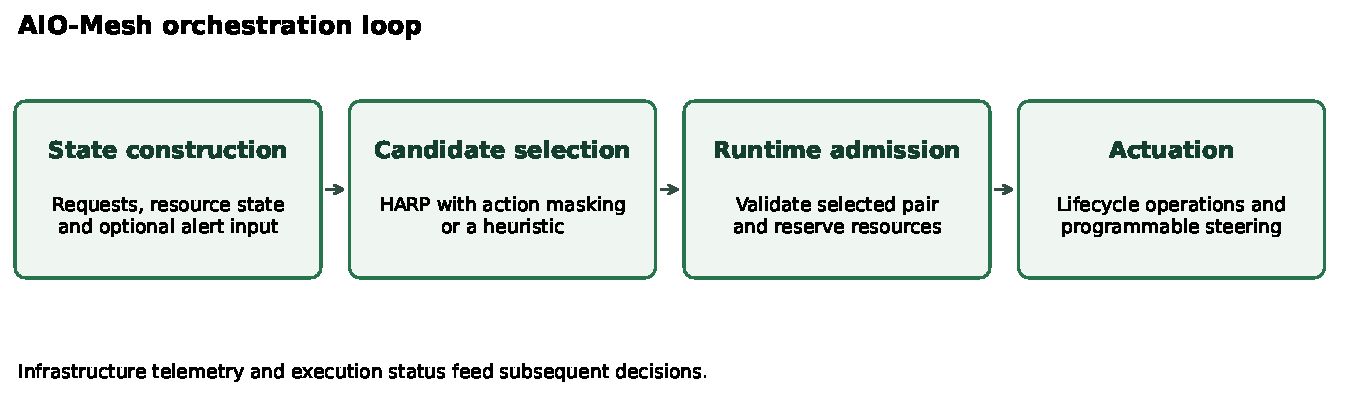
\includegraphics[width=\linewidth]{figs/overview.pdf}
    \caption{\newrev{AIO-Mesh closed-loop architecture connecting telemetry, candidate selection, local admission, cloud-native lifecycle operations, and programmable steering. HARP is a replaceable candidate-selection component. The implemented admission predicates and their relationship to forwarding realization are described in the text.}}
    \label{fig:aio_mesh_architecture}
\end{figure*}

\subsection{Closed-Loop Runtime Organization}
\label{subsec:architecture_overview}

The AIO-Mesh runtime follows an observe--decide--admit--actuate--verify loop. The telemetry layer collects resource, service, orchestration, and data-plane signals, including CPU and memory pressure, active VNF placement, service-chain demand, alert state, SRv6 steering status, and MSD-related counters. The state manager normalizes these signals and constructs the policy-facing graph state defined in \autoref{sec:system_model}. This state is passed to the policy runtime together with the substrate topology.

The policy runtime hosts two decision paths. Under stable load, AIO-Mesh may use a deterministic heuristic path to reduce overhead. Under stress \rev{or an active alert}, it invokes HARP to produce a topology-aware \rev{placement--routing proposal}. The heuristic and learned paths share the same safety boundary; neither path is allowed to actuate directly. This design makes the learned policy replaceable or retrainable without changing the admission contract of the system.

\rev{The Hybrid runtime selects between these paths using hysteresis. Let \(A_t\in\{0,1\}\) indicate an active alert and \(u_t=\max(\bar{u}^{CPU}_t,\bar{u}^{MSD}_t)\), where the terms denote mean normalized CPU utilization and the runtime's MSD accounting indicator. The decision mode is}
\begin{equation}
\rev{\mathrm{mode}_{t+1}=
\begin{cases}
\mathrm{HARP}, & u_t>0.45\ \lor\ A_t=1,\\
\mathrm{heuristic}, & u_t<0.35\ \land\ A_t=0,\\
\mathrm{mode}_t, & \text{otherwise}.
\end{cases}}
\label{eq:hybrid_gate}
\end{equation}
\rev{The MSD indicator is a policy-side accounting feature, not parser capacity consumed across flows. The gate does not implement an additional dwell-time rule or an independently evaluated forecasting model.}

The admission layer is the boundary between decision making and infrastructure modification. It validates the candidate action against residual compute and memory capacity, \rev{checks the available MSD predicate for the proposed placement--routing pair}, and determines whether the action can proceed to actuation. A feasible action is admitted and passed to the actuation layer. An infeasible action is rejected before deployment or steering, and if no feasible action remains \rev{in the searched candidate set}, the runtime returns \texttt{NO\_SAFE\_ACTION}.

The actuation layer translates admitted decisions into cloud-native and network-control operations. Kubernetes and workflow automation are used to deploy, reuse, scale, or migrate VNFs. The SRv6/P4 interface generates steering state, installs the corresponding forwarding rules, and reports steering confirmation or data-plane anomalies. These post-actuation signals are fed back to the telemetry layer, closing the AIOps loop.

\subsection{Policy Runtime and State Management}
\label{subsec:policy_runtime}

AIO-Mesh treats HARP as an operational policy artifact rather than as an isolated model file. The runtime therefore manages the trained policy, topology descriptor, normalization state, safety configuration, and controller endpoints as a consistent deployment unit. This is necessary because an otherwise valid policy can become unsafe if it is executed with stale topology information, inconsistent preprocessing, or an incompatible data-plane profile.

The state manager maintains the deployed observation contract. It maps heterogeneous telemetry into a fixed graph-structured state containing node features, global request features, and the substrate adjacency matrix. The same contract is used for HARP inference and for runtime admission logging. For each decision, AIO-Mesh records the request context, selected action, feasibility outcome, rejection reason if applicable, and post-actuation feedback. These logs allow operators to distinguish policy unavailability, lack of feasible actions, controller failure, and data-plane violation.

This runtime organization follows an MLOps discipline but is specialized for network operations. Model versioning, preprocessing consistency, and observability are not sufficient by themselves; the policy also needs a fail-closed safety boundary because its output changes infrastructure state. AIO-Mesh therefore does not silently push a learned decision when the model, topology descriptor, normalization state, or controller endpoint is unavailable or inconsistent. In such cases, the runtime either falls back to a verified safety-preserving heuristic path or returns an explicit rejection.

\subsection{Safety Boundary and Admission Semantics}
\label{subsec:safety_boundary}
\label{subsec:freshness_revalidation}

The safety boundary enforces the distinction between candidate decisions and admitted infrastructure actions. A candidate action may be generated by HARP or by the heuristic path, but it becomes operational only after passing the hard feasibility checks. CPU and memory feasibility are checked against residual node capacity. SRv6 feasibility is checked \rev{against the implemented local MSD predicate; feasibility of the complete realized SID list additionally requires the condition in Eq.~\eqref{eq:realization_soundness}}.

\rev{Admission checks and reserves the selected pair under a process-level lock, serializing local reservations. The reservation rejects a snapshot-version mismatch under that lock. This does not provide an atomic transaction across Kubernetes and P4 or consistency with external controllers. Telemetry age measures time since local ingestion; upstream measurement freshness is not established. Accordingly, safety at commitment is conditional on the accuracy of the checked predicates and the validity of the checked state until commitment. Policy-side masking does not replace this independent admission step.}

This design gives the runtime \rev{fail-closed behavior for the checked predicates}. If the feasible action set is empty, the result is \texttt{NO\_SAFE\_ACTION}, not best-effort deployment. If steering confirmation is not received, the previous service path is preserved \rev{in the intended make-before-break workflow}. If a replacement VNF cannot be verified during migration, the old instance is not removed. If an unexpected MSD-drop counter is observed after actuation, the decision context is logged \rev{for subsequent diagnosis}.

The distinction between an unsafe candidate and an admitted violation is central to AIO-Mesh. Under overload, many candidate decisions may be infeasible because the infrastructure has exhausted safe compute or SID-depth headroom. This is not itself a safety failure. The failure occurs only when such a candidate is admitted and installed in the data plane. AIO-Mesh is therefore designed to convert unsafe candidates into explicit admission rejections before they become data-plane behavior.

\sloppy
\rev{The logical decision record distinguishes \texttt{REJECTED}, \texttt{ADMITTED}, \texttt{DEPLOYED}, and \texttt{FAILED}. Admission and reservation authorize execution; they do not establish successful deployment or steering.}

\newrev{The orchestration service constructs a bounded SID list using the placement node, repeated routing anchor, and requested SID count before calling the local pair-reservation predicate. It does not separately realize a complete chain, reconcile per-function resources, or validate the full forwarding path. Admission success therefore does not establish deployment or forwarding success.}

\subsection{Cloud-Native Lifecycle Actuation}
\label{subsec:cloud_native_actuation}

For admitted actions, AIO-Mesh invokes cloud-native lifecycle operations. A new service-chain request may require creating one or more VNFs, reusing existing instances, exposing service endpoints, and preparing steering state. A migration action follows a stricter make-before-break sequence. The replacement VNF is created first, Kubernetes readiness is verified, the new endpoint is translated into an \rev{SRv6 service path}, and the controller installs the new steering state. Only after steering confirmation can the old instance be removed. \rev{Admission must account for the temporary resource overlap between old and replacement instances.}

This separation keeps responsibilities clear. The policy selects an \rev{orchestration proposal}; the lifecycle layer executes deployment and migration workflows; and the SRv6/P4 controller realizes the forwarding behavior. \rev{Make-before-break sequencing preserves lifecycle ordering; packet-level zero-downtime migration is outside the evaluated scope.}

\subsection{Programmable Data-Plane Interface}
\label{subsec:data_plane_interface}
The request helper creates a bounded list with \(\max(1,\mathrm{msd\_req})\) entries derived from the selected placement and routing anchor. This is not an expansion of every VNF placement and every inter-function substrate path. The lifecycle and SDN adapters provide deployment and steering operations, but the implemented interface does not establish a per-request mapping from the formal chain to the packet path.

\newrev{The orchestration API returns the admitted synthetic list, but the migration steering service does not consume it. That service independently constructs an endpoint SID and fixed steering rules, so the checked SID list is not linked to the installed packet path. The orchestration endpoint schedules lifecycle work only on the DRL branch with a forecast alert; a separate direct P4-rule endpoint bypasses pair admission. The local admission result therefore does not apply to every actuation interface.}

\newrev{A local reservation does not establish successful Kubernetes deployment, steering installation, or packet forwarding. Those outcomes require request-correlated controller logs and packet or counter observations. Binding SID compression, general path reconstruction, and a candidate-path cache are not implemented features of the prototype.}

\subsection{End-to-End Request Lifecycle}
\label{subsec:request_lifecycle}
Algorithm~\ref{alg:aiomesh_lifecycle} summarizes the pair-selection service. The HTTP router handles telemetry and forecast inputs and schedules lifecycle work separately. Returning a selected and reserved pair does not establish that deployment or steering completed.

\begin{algorithm}[t]
\caption{Local pair-selection and reservation service}
\label{alg:aiomesh_lifecycle}
\small
\begin{algorithmic}[1]
\Require Request \(q\), local state manager, heuristic and DRL proposal providers
\Ensure Selected pair with local reservation, or rejection
\State \(mode\gets\textsc{ChooseMode}()\) using Eq.~\eqref{eq:hybrid_gate}
\If{\(mode=\mathrm{heuristic}\)}
    \State Attempt heuristic pair selection
    \State On hard-constraint failure, request a DRL/fallback proposal
\Else
    \State Request a DRL/fallback proposal
\EndIf
\State Build bounded SID list from the selected pair and requested depth
\State Check and reserve the pair under the local process lock
\If{reservation fails and the proposal was heuristic}
    \State Obtain one DRL/fallback proposal; rebuild SID list; retry reservation
\EndIf
\If{reservation fails}
    \State \Return \texttt{NO\_SAFE\_ACTION}
\EndIf
\State \Return Pair, bounded SID list, branch label and local reservation
\end{algorithmic}
\end{algorithm}

\newrev{The router may schedule deployment or migration after this service returns. The service does not provide a complete-chain realization token or a transaction across Kubernetes and P4. The current HTTP success response and branch label alone do not certify model inference, successful actuation, or forwarding.}

\section{HARP: Hardware-Aware Reinforcement Policy}
\label{sec:harp}

HARP is the learned decision engine inside AIO-Mesh. Its objective is to select high-quality orchestration actions while preserving the hard deployability constraints defined in \autoref{sec:system_model}. The key design principle is to separate \emph{hard feasibility} from \emph{soft optimization}. CPU, memory, and SRv6 MSD feasibility are \rev{considered during policy masking and independently checked by runtime admission} before actuation. Latency, SLA pressure, load balance, and \rev{action-switching overhead} are optimized through the reward function. \rev{The policy-side mask filters locally infeasible proposals; runtime admission retains authority to reject actions before deployment.}

HARP combines three mechanisms: a graph-attention encoder for topology-aware state representation, masked policy optimization for hard constraints, and adaptive penalties for soft operational objectives. The selected action is not applied directly to the infrastructure. It is returned to the AIO-Mesh runtime, which performs final admission validation, lifecycle actuation, and SRv6/P4 steering.

\subsection{MDP Formulation}
\label{subsec:harp_mdp}

We formulate online service-chain orchestration as a Markov Decision Process
$ \rev{\mathcal{M}=(\mathcal{S},\mathcal{A},\mathcal{P},r,\gamma),}$
where \(\mathcal{S}\) is the state space, \(\mathcal{A}\) is the action space, \(\mathcal{P}\) denotes the transition dynamics induced by traffic arrivals and infrastructure updates, \rev{\(r\)} is the reward function, and \(\gamma\) is the discount factor.

At decision epoch \(t\), the state is $ s_t=(\mathbf{X}_t,\mathbf{g}_t,\mathcal{A}_{topo}),$
where \(\mathbf{X}_t\in\mathbb{R}^{N\times 6}\) is the node-feature matrix, \(\mathbf{g}_t\in\mathbb{R}^{13}\) contains request-level and global operational features, and \(\mathcal{A}_{topo}\) is the substrate adjacency matrix. This state representation follows the system model in Section~\ref{sec:system_model}: runtime dynamics are encoded in the node and global features, while the physical topology is preserved as a graph prior.

The abstract orchestration action in Section~\ref{sec:system_model} couples placement, routing, and operational mode. \rev{In the implemented policy, HARP selects a placement--routing pair \(a_t=(v_t^{place},v_t^{route})\), encoded as}
\begin{equation}
\rev{\hat a_t=v_t^{place}N+v_t^{route},\quad \hat a_t\in\{0,\ldots,N^2-1\}.}
\label{eq:harp_action_encoding}
\end{equation}
\rev{The pair is decoded as \(v_t^{place}=\lfloor\hat a_t/N\rfloor\) and \(v_t^{route}=\hat a_t\bmod N\), giving \(|\mathcal A|=N^2\). It does not enumerate every function placement or encode a migration mode. The runtime realizes the pair using the request and deployment context. The main v11 checkpoints were trained with a factorized \(\mathrm{MultiDiscrete}([N,N])\) head, not a flat \(N^2\)-logit head. At inference, the adapter forms pair logits \(z_{p,r}=z^{place}_{p}+z^{route}_{r}\), then applies the flat pair mask. This conversion preserves the unmasked factorized action distribution; it does not imply that the original training used pair-level masking.}

HARP does not enumerate packet-level forwarding rules. Instead, \rev{the policy evaluates local placement--routing feasibility and passes its proposal to the runtime for admission. The complete realized path and SID-list feasibility are not certified by the pair-level policy alone.}

\subsection{Graph-Attention State Encoder}
\label{subsec:harp_gat}

\rev{A flat state encoder does not explicitly model the neighborhood structure of the substrate}, whereas service-chain orchestration depends on topological relations among source, destination, candidate service locations, and routing anchors. HARP therefore uses a graph-attention encoder to represent the substrate topology and runtime node state~\cite{velickovic2018graph}.

Let \rev{\(\mathbf{H}^{(0)}=\bar{\mathbf{X}}_t\), where \(\bar{\mathbf X}_t\) contains the normalized node features defined below.} For attention head \(k\), the unnormalized attention coefficient from node \(j\) to node \(i\) is
\begin{equation}
    e_{ij}^{(k)}
    =
    \mathrm{LeakyReLU}
    \left(
    \mathbf{a}_{k}^{\top}
    [\mathbf{W}_{k}\mathbf{h}_i \Vert \mathbf{W}_{k}\mathbf{h}_j]
    \right),
    \quad j\in\mathcal{N}(i),
\end{equation}
and the normalized attention weight is
\begin{equation}
    \alpha_{ij}^{(k)}
    =
    \frac{\exp(e_{ij}^{(k)})}
    {\sum_{r\in\mathcal{N}(i)}\exp(e_{ir}^{(k)})}.
\end{equation}
The updated node representation is
\begin{equation}
    \mathbf{h}'_i
    =
    \mathop{\Vert}_{k=1}^{K}
    \sigma
    \left(
    \sum_{j\in\mathcal{N}(i)}
    \alpha_{ij}^{(k)}\mathbf{W}_{k}\mathbf{h}_j
    \right),
\end{equation}
where \(K\) is the number of attention heads and \(\sigma(\cdot)\) is a nonlinear activation. After \(L\) graph-attention layers, the graph embedding is pooled and concatenated with global request features:
\begin{equation}
\mathbf{z}_t=[\mathrm{Pool}(\mathbf{H}^{(L)})\Vert\rev{\bar{\mathbf{g}}_t}].
\end{equation}
The vector \(\mathbf{z}_t\) is passed to the actor and critic heads. \rev{Here, \(\bar{\mathbf g}_t\) denotes the normalized global features.}

\rev{The six node features comprise CPU utilization, memory utilization, an MSD accounting ratio and its complement, a CPU-alert flag, and normalized geographic context. The thirteen global features comprise three demand features, five service-type indicators, and five aggregate/context features. CPU and memory percentages are scaled by 100, MSD indicators use configured profile limits, and the assembled observation is clipped to \([0,1]\). These MSD features are policy-side proxies, not physical SID-depth validation.}

\rev{The saved normalizer subsequently applies}
\begin{equation}
\rev{\bar{x}_j=\mathrm{clip}\left(\frac{x_j-\mu_j}{\sqrt{\sigma_j^2+\epsilon_{norm}}},-c,c\right),}
\end{equation}
\rev{where \(\mu_j\) and \(\sigma_j^2\) are training-derived statistics. \rev{Inference uses the checkpoint's saved normalizer with frozen statistics.}}

\subsection{Hard-Feasibility Action Mask}
\label{subsec:harp_masking}

The central \rev{policy-side feasibility mechanism} in HARP is the hard-feasibility mask. Let \(\mathcal{F}_{loc}(s_t)\subseteq\mathcal{A}\) denote the \rev{locally feasible} action set at state \(s_t\):
\begin{equation}
\rev{\begin{aligned}
\mathcal{F}_{loc}(s_t)=\{a\in\mathcal A\mid
&C_{cpu}^{loc}(a,s_t)=0,\ C_{mem}^{loc}(a,s_t)=0,\\
&C_{msd}^{loc}(a,s_t)=0\}.
\end{aligned}}
\label{eq:feasible_set}
\end{equation}
Here \(C_{cpu}^{loc}\), \(C_{mem}^{loc}\), and \(C_{msd}^{loc}\) denote implementation-level checks, rather than a proof of the full-chain constraints. The current simulator and runtime use a flat \(N^2\) pair mask. Main checkpoints have a factorized \(2N\)-logit output head, which is converted to pair logits before runtime masking. \newrev{The revised algorithm benchmark evaluates the retained main checkpoints through this adapter; the ablation uses separate flat-action checkpoints.}

\newrev{The runtime's local node predicate currently checks CPU and memory increments and an accumulated MSD accounting value. For node \(u\), its implemented check includes}
\begin{equation}
\begin{aligned}
M^{node}_t(u)=\mathbb I[&b^{cpu}_{u,t}+d_q^{cpu}\le c_u^{cpu}\\
&\land b^{mem}_{u,t}+d_q^{mem}\le c_u^{mem}\\
&\land b^{msd}_{u,t}+\mathrm{msd\_req}\le m_u^{msd}].
\end{aligned}
\label{eq:runtime_pair_mask}
\end{equation}
\newrev{Admission applies this predicate to both touched nodes and increments their accounting state, counting a coincident placement/route node once. This differs from per-list parser-depth feasibility: MSD is not a resource consumed across flows. The simulation additionally uses a hop-dependent MSD estimate. Neither representation by itself establishes the formal per-profile SID-depth condition in Eq.~\eqref{eq:msd_constraint}. Our safety conclusions are limited to the implemented checks.}

The policy mask is built at inference time from the locally observed state; there is no verified telemetry-version or freshness-TTL contract spanning masking, reservation and actuation.

The actor produces a logit \(z_a\) for each action \(a\in\mathcal{A}\). HARP applies the binary mask
\begin{equation}
M_t(a)=
\begin{cases}
1, & \rev{a\in\mathcal{F}_{loc}(s_t)},\\
0, & \rev{a\notin\mathcal{F}_{loc}(s_t)},
\end{cases}
\end{equation}
and replaces infeasible logits by \(-\infty\):
\begin{equation}
\tilde{z}_a=
\begin{cases}
z_a, & M_t(a)=1,\\
-\infty, & M_t(a)=0.
\end{cases}
\end{equation}
The masked policy is then
\begin{equation}
\pi_\theta^{M}(a\mid s_t)=\frac{\exp(\tilde{z}_a)}{\sum_{b\in\mathcal{A}}\exp(\tilde{z}_b)}.
\end{equation}

\sloppy
HARP optimizes this masked policy using PPO~\cite{schulman2017proximal}. With
\begin{equation}
    \rho_t(\theta)=
    \frac{\pi_\theta^{M}(a_t\mid s_t)}
    {\pi_{\theta_{old}}^{M}(a_t\mid s_t)},
\end{equation}
the clipped objective is
% \begin{equation}
% \mathcal{L}^{CLIP}(\theta)=\mathbb{E}_t\left[\min\left(\rho_t(\theta)\hat{A}_t,\mathrm{clip}(\rho_t(\theta),1-\epsilon_{PPO}, \\
% 1+\epsilon_{PPO})\hat{A}_t\right)\right],
% \end{equation}
\begin{equation} \label{eq:ppo_clip} \mathcal{L}^{\mathrm{CLIP}}(\theta) = \mathbb{E}_t \left[ \min \left\{ \begin{aligned} &\rho_t(\theta)\hat{A}_t,\\ &\operatorname{clip}\!\left( \rho_t(\theta), 1-\epsilon_{\mathrm{PPO}}, 1+\epsilon_{\mathrm{PPO}} \right)\hat{A}_t \end{aligned} \right\} \right]. \end{equation}
with standard value and entropy terms added during training. This masking mechanism is related to invalid action masking in policy-gradient methods~\cite{huang2022closer}, \rev{but policy masking alone does not guarantee the correctness of a subsequently realized forwarding action}.

\subsection{Reward for Soft Operational Objectives}
\label{subsec:harp_penalty}

HARP uses the reward function \rev{to rank locally feasible actions and penalize operational costs}. Latency, \rev{action switching}, SLA pressure, and load balance affect service quality, but they do not by themselves determine whether an action is physically deployable. \rev{The implemented training reward is}
\begin{equation}
\rev{\begin{aligned}
r_t&=-20, \hspace{36mm} \text{if the action is invalid};\\
r_t&=100+0.25d_q^{msd}d_q^{cpu}+30I_{core,elephant}\\
&\quad+15I_{v^{place}\ne v^{route}}-10I_{switch}-w_{svc}L_t\\
&\quad+\lambda_t\frac{L_t}{T_{svc}}I_{L_t>T_{svc}}-50I_{alert}+\rho_{msd}I_{msd}, \text{otherwise}.
\end{aligned}}
\label{eq:harp_reward}
\end{equation}
\rev{Here, \(I_{switch}\) indicates a change of placement--routing pair, \(I_{core,elephant}\) rewards a configured core node for Elephant traffic, and \(w_{svc}\) and \(T_{svc}\) are service-class latency parameters. The configured thresholds for IoT, Video, VoIP, Data, and Attack are 30, 50, 100, 10, and 500 ms, respectively. The MSD coefficient satisfies \(\rho_{msd}\le0\), with default value \(-50\). In protected configurations, hard admission remains independent of this reward term.}

The SLA penalty multiplier is adapted from recent violation behavior:
\begin{equation}
\rev{\lambda_{k+1}=\mathrm{clip}\left(\lambda_k-\eta_\lambda(\bar{V}_k-\tau),-3000,-5\right),}
\label{eq:lambda_update}
\end{equation}
\rev{where \(\bar V_k\) is the reported violation rate averaged by the training callback, \(\tau=0.015\), \(\eta_\lambda=10\), and the initial multiplier is \(-100\). The environment uses a 20-step rolling violation indicator. The negative sign convention increases the penalty magnitude when violations exceed the target.}

This adaptive penalty regulates soft service-level pressure without weakening hard deployability constraints. \rev{The adaptive update is a reward-shaping heuristic rather than a constrained-RL safety guarantee. }

\subsection{Admission and Migration Semantics}
\label{subsec:harp_admission}
An empty feasible set requires explicit rejection or a guarded fallback that still passes admission. The inference path includes a fallback for unavailable models or inference exceptions; it does not establish a dedicated all-false-mask rejection branch. Shadow mode is also supported and is distinct from inference using a trained checkpoint.

Migration is orchestrated by the lifecycle layer rather than emitted as a separate HARP action. The control flow specifies readiness and steering order, but does not establish packet-level continuity or rollback outcomes.

\subsection{Decision Procedure}
\label{subsec:harp_decision_procedure}
\begin{algorithm}[t]
\caption{Runtime inference path for a factorized policy checkpoint}
\label{alg:harp_decision}
\small
\begin{algorithmic}[1]
\Require Request, local state, model configuration and saved normalizer
\Ensure Proposal with inference/fallback status; not a deployment outcome
\State Load checkpoint and matching normalizer; convert a legacy \(2N\) action head to additive \(N^2\) pair logits
\If{shadow mode}
    \State Return simulated proposal; this is not learned-policy evidence
\ElsIf{model unavailable}
    \State Return safe-search fallback or propagate hard-constraint failure
\EndIf
\State Build observation and apply the available saved normalizer
\State Build the runtime pair mask of length \(N^2\)
\State Predict a masked flat action and decode the placement--routing pair
\State On inference exception, use the guarded fallback path
\State Pass the proposal to independent local admission in Algorithm~\ref{alg:aiomesh_lifecycle}
\end{algorithmic}
\end{algorithm}

\paragraph{Computational complexity}\label{subsec:harp_complexity}
The main actor produces \(2N\) logits; its runtime adapter expands them into \(N^2\) additive pair scores, and the pair mask requires \(\Theta(N^2)\) storage and score construction. The current flat simulator actor produces \(N^2\) logits directly. The graph-encoding term depends on the actual encoder, adjacency representation and attention implementation. These dimensional bounds do not establish measured latency, throughput, or end-to-end scalability.

\section{Experiments and Evaluation}
\label{sec:evaluation}
\newrev{We evaluate three aspects of the orchestration design: the acceptance achieved by alternative policies under a common admission boundary; the contributions of policy representation, masking, and admission; and sensitivity to offered intensity and background occupancy. The three-workload benchmark establishes policy effectiveness under long-lived stress traffic. Ablation separates candidate selection from admission, while timing measurements quantify simulator decision cost. Load and occupancy sweeps then examine whether the policy comparison changes under different resource-pressure regimes. Table~\ref{tab:evaluation_protocols} summarizes the protocols and their measurement boundaries.}

\subsection{\newrev{Experimental Setup}}
\label{subsec:experimental_setup}
\newrev{The algorithm benchmark evaluates fixed, topology-specific main-policy checkpoints and their observation normalizers; no model is retrained during evaluation. It covers the 10-node Vietnam, 14-node NSFNET, and 23-node GEANT2 topologies under the stress load (arrival rate 1.0; request TTL 100--500). The three tested workloads are Elephant stress (mapped to Heavy-tail), Burst surge (mapped to Bursty), and a separately configured Chaos workload. Each algorithm--topology--workload condition uses 20 evaluation seeds, \{42, 100, 2024, 8888, 9999, 7, 17, 73, 314, 2718, 11, 23, 47, 89, 101, 211, 512, 1024, 4096, 8192\}, and 3,000 simulator steps per seed. Algorithms share the offered-request trace within each seed; for the Bursty workload, the generator repeats the same trace across seeds.}

\newrev{The Greedy baseline selects the node with the most residual CPU capacity, then the routing node with minimum latency among nodes distinct from the placement node. Decoupled AI selects the least-loaded-CPU placement and then a neighboring node with the least RAM load. SAF-H filters placement--routing pairs using CPU, memory, bandwidth, and MSD checks, then selects the pair minimizing a weighted sum of latency, CPU utilization, and hop count (weights 0.5, 100, and 5, respectively). Each algorithm is evaluated with protected and unprotected admission; the acceptance results below report the protected mode. The matched-trace ablation separately evaluates variant-specific checkpoints on Vietnam, NSFNET, and GEANT2 using 20 seeds and 3,000 simulator steps per seed--workload cell.}

\newrev{The named substrates use the node locations and configured resource profiles associated with Vietnam, NSFNET, and GEANT2. Simulator adjacency is derived by thresholding coordinate-based pair latencies rather than importing the physical backbone edge lists. The evaluated adjacency has 45, 91, and 253 undirected edges, respectively: all three are complete graphs at these settings. Consequently, these experiments vary node count and geographic/resource profiles, but do not establish generalization across the physical connectivity of the corresponding operational backbones.}

\begin{table*}[t]
\centering
\caption{\newrev{Protocols supporting the simulation evaluation. All use 20 evaluation seeds and 3,000 simulator steps per seed and condition. Main-policy and ablation checkpoints are distinct.}}
\label{tab:evaluation_protocols}
{\color{ForestGreen}
\scriptsize
\begin{tabular}{p{0.18\textwidth}p{0.19\textwidth}p{0.25\textwidth}p{0.28\textwidth}}
\toprule
Experiment & Checkpoint/interface & Offered traffic and occupancy & Interpretation \\
\midrule
Algorithm benchmark & Main, factorized head with pair adapter & Three stress workloads; arrival 1.0; TTL 100--500 & Protected policy comparison; both admission modes recorded \\
Matched-trace ablation & Variant-specific flat-action policies & Four workloads; arrival 1.0; TTL 100--500 & Candidate quality, pruning, and modeled admission; distinct trained variants \\
Timed ablation & Variant-specific flat-action policies & Ten topology--workload conditions; arrival 1.0; TTL 100--500 & Simulator normalization, inference, and stepping; external actuation excluded \\
Background chains & Main with pair adapter & Bursty; arrival 1.0; 0/25/50/100 persistent chains; topology-scaled TTL & Occupancy sensitivity under a separate resource-pressure protocol \\
Load-sweep protocol & Main with pair adapter & Seven multipliers 0.2--1.5; arrival capped at 1.0; demand/TTL scaled above 1.0 & Combined offered-intensity stress across three substrates \\
\bottomrule
\end{tabular}}
\end{table*}

\subsection{\newrev{Baselines, Ablation Variants, and Metrics}}
\label{subsec:baselines_metrics}
\newrev{Decoupled AI is the benchmark name for a sequential CPU/RAM heuristic. SAF-H searches feasible placement--routing pairs using the cost defined above. The main benchmark evaluates factorized-action HARP checkpoints through the pair adapter, while ablation evaluates separately trained flat-action variants. Comparisons are therefore made within each experiment, with checkpoint and action interface held to the corresponding protocol.}

\newrev{The algorithm benchmark reports acceptance per offered, non-skipped request and aggregates 20 seed-level rates with population standard deviation. For HARP versus SAF-H, paired seed-level acceptance differences are tested using the two-sided Wilcoxon signed-rank test; percentile bootstrap 95\% confidence intervals use 10,000 resamples, and Holm correction is applied across the nine topology--workload comparisons. The paired rank-biserial effect is positive when HARP tends to have higher acceptance; it describes the signed rank balance, not the magnitude in percentage points. The timing-instrumented ablation reports safe acceptance and policy-decision p95 over 20 evaluation seeds using mean and sample standard deviation. The matched-trace ablation reports sample standard deviation across seed--workload evaluation cells. These deviations describe evaluation variation conditional on the evaluated checkpoints, not variation across independently trained policies.}

\newrev{For the timing-instrumented and matched-trace ablations, safe acceptance is accepted requests minus the unique admitted requests violating any modeled hard CPU, memory, bandwidth, or MSD constraint, divided by offered non-skipped requests. Proposed CPU, memory, bandwidth, and MSD violation rates may overlap; the union rate is reported separately. Candidate pruning is computed over the flat $N^2$ action set.}

\newrev{All simulation rates use offered, non-skipped requests as the request denominator unless stated otherwise. Runtime rejection and admitted violation are separate outcomes; neither is a measure of successful physical deployment. Algorithm-benchmark comparisons pair policies by topology, workload, and seed and verify identical offered-trace hashes. The matched-trace ablation likewise reuses the offered trace across variants, although policy-dependent admissions can cause simulated state trajectories to diverge.}

\subsection{\newrev{Hardware-Safe Admission under Workload Saturation}}
\newrev{All four algorithms use the same simulator admission checks in protected mode. Across nine topology--workload conditions, each policy is evaluated for 540,000 simulator steps and records zero admitted modeled hard violations. The common result demonstrates the role of admission across candidate-selection methods. Policy effectiveness is assessed separately through acceptance and the paired HARP--SAF-H differences in Figure~\ref{fig:benchmark_effects}.}

\begin{figure*}[t]
\centering
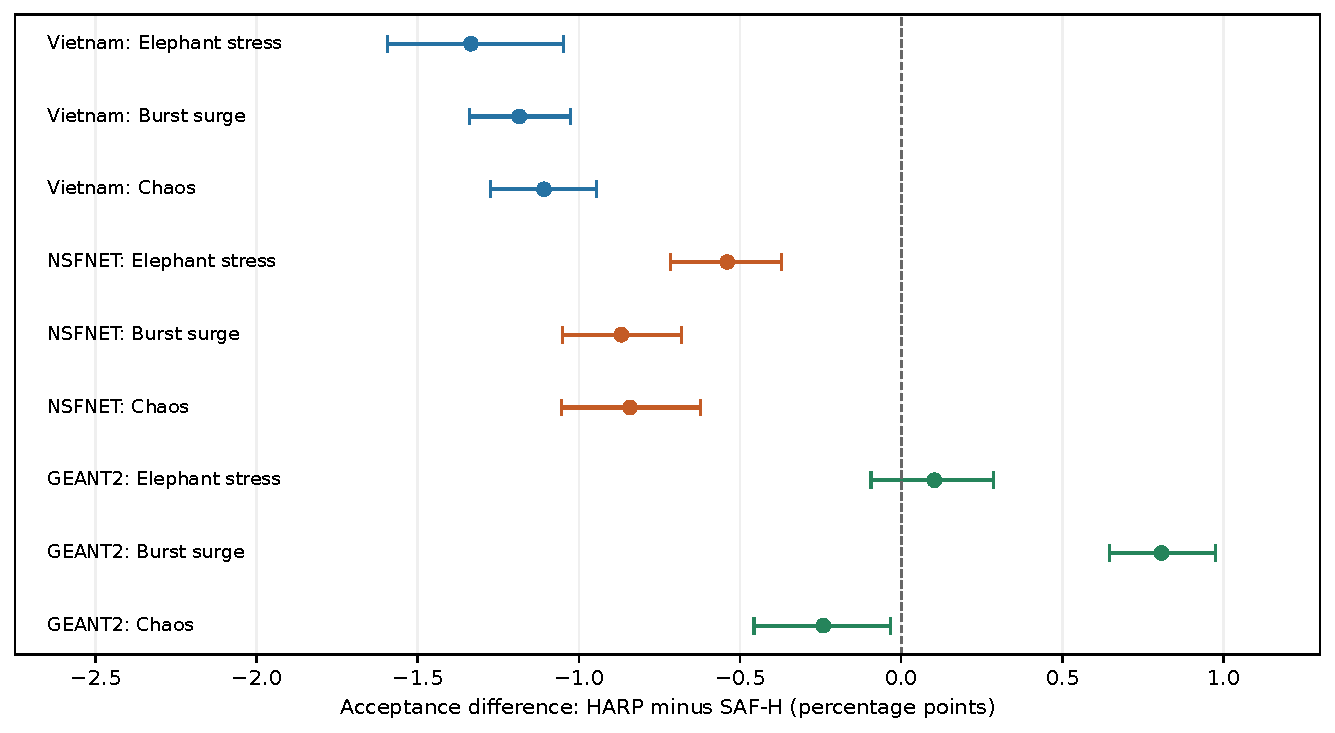
\includegraphics[width=0.94\textwidth]{figs/benchmark_paired_effects.pdf}
\caption{\newrev{Protected HARP minus SAF-H acceptance across three topologies and three stress workloads. Points show mean paired seed-level differences; horizontal intervals are percentile-bootstrap 95\% confidence intervals from paired seed-level trials. Positive values favor HARP. Holm-adjusted tests across all nine conditions are reported in Table~\ref{tab:benchmark_paired_statistics}.}}
\label{fig:benchmark_effects}
\end{figure*}

\subsection{\newrev{Simulation Results across Distributed Topologies}}
\label{subsec:simulation_results}
\newrev{Table~\ref{tab:simulation_acceptance_summary} reports mean acceptance over 20 evaluation seeds for the protected versions of four algorithms. Each topology--workload cell contains 20 paired seed-level trials of 3,000 simulator steps; policies share offered traces within each seed, while the Bursty generator repeats the same offered trace across seeds. Acceptance is not a full-chain safety metric.}

\begin{table}[t]
\centering
\caption{\newrev{Protected-policy acceptance (\%; 20 seeds, mean $\pm$ population SD). Profiles: E = Elephant stress, B = Burst surge, C = Chaos; DAI = Decoupled AI.}}
\label{tab:simulation_acceptance_summary}
\scriptsize
{\color{ForestGreen}
\setlength{\tabcolsep}{3pt}
\resizebox{\columnwidth}{!}{%
\begin{tabular}{llrrrr}
\toprule
Network & Profile & Greedy & DAI & SAF-H & HARP \\
\midrule
Vietnam & E & 44.07 $\pm$ 0.56 & 44.30 $\pm$ 0.60 & 44.34 $\pm$ 0.67 & 42.97 $\pm$ 0.63 \\
Vietnam & B & 58.78 $\pm$ 0.41 & 58.78 $\pm$ 0.46 & 58.84 $\pm$ 0.61 & 57.65 $\pm$ 0.52 \\
Vietnam & C & 45.04 $\pm$ 0.53 & 45.03 $\pm$ 0.64 & 45.08 $\pm$ 0.63 & 43.63 $\pm$ 0.47 \\
NSFNET & E & 52.64 $\pm$ 0.53 & 52.64 $\pm$ 0.53 & 52.66 $\pm$ 0.42 & 51.73 $\pm$ 0.54 \\
NSFNET & B & 68.27 $\pm$ 0.31 & 68.27 $\pm$ 0.31 & 68.28 $\pm$ 0.33 & 66.85 $\pm$ 0.55 \\
NSFNET & C & 53.73 $\pm$ 0.68 & 53.73 $\pm$ 0.68 & 53.82 $\pm$ 0.65 & 52.59 $\pm$ 0.72 \\
GEANT2 & E & 64.73 $\pm$ 0.46 & 64.71 $\pm$ 0.46 & 64.67 $\pm$ 0.39 & 64.61 $\pm$ 0.48 \\
GEANT2 & B & 79.64 $\pm$ 0.24 & 79.64 $\pm$ 0.24 & 79.68 $\pm$ 0.26 & 80.64 $\pm$ 0.39 \\
GEANT2 & C & 66.60 $\pm$ 0.47 & 66.60 $\pm$ 0.47 & 66.70 $\pm$ 0.49 & 66.50 $\pm$ 0.60 \\
\bottomrule
\end{tabular}%
}
}
\end{table}

\newrev{All four protected algorithms recorded zero admitted hard violations in all nine reported simulator conditions. HARP had lower mean acceptance than Greedy, Decoupled AI, and SAF-H in every Vietnam and NSFNET workload. On GEANT2, HARP exceeded SAF-H in Burst surge, was lower in Elephant stress and Chaos, and the Elephant-stress difference was not statistically significant after correction. Table~\ref{tab:benchmark_paired_statistics} reports all nine paired HARP--SAF-H comparisons with Holm correction. These results show that the protected HARP checkpoint did not consistently improve acceptance over the baselines across topologies and workloads. The matched-trace ablation below separately evaluates candidate masking and local admission.}

\begin{table}[t]
\color{ForestGreen}
\centering
\caption{\newrev{HARP--SAF-H acceptance differences ($\Delta$, percentage points; 20 paired seeds). Intervals: bootstrap 95\% CI; $p_H$: Wilcoxon $p$ with Holm correction across nine conditions; $r$: rank-biserial effect. Profiles E/B/C follow Table~\ref{tab:simulation_acceptance_summary}.}}
\label{tab:benchmark_paired_statistics}
\scriptsize
\setlength{\tabcolsep}{3pt}
\resizebox{\columnwidth}{!}{%
\begin{tabular}{llrrrr}
\toprule
Network & Profile & $\Delta$ & 95\% CI & $p_H$ & $r$ \\
\midrule
Vietnam & E & $-1.373$ & [$-1.663$, $-1.055$] & $1.72\times 10^{-5}$  & $-0.990$ \\
Vietnam & B & $-1.193$ & [$-1.368$, $-1.023$] & $1.72\times 10^{-5}$  & $-1.000$ \\
Vietnam & C & $-1.447$ & [$-1.687$, $-1.197$] & $1.72\times 10^{-5}$  & $-1.000$ \\
NSFNET & E & $-0.928$ & [$-1.073$, $-0.783$] & $1.72\times 10^{-5}$  & $-1.000$ \\
NSFNET & B & $-1.427$ & [$-1.657$, $-1.197$] & $1.72\times 10^{-5}$  & $-1.000$ \\
NSFNET & C & $-1.228$ & [$-1.417$, $-1.048$] & $1.72\times 10^{-5}$  & $-1.000$ \\
GEANT2 & E & $-0.058$ & [$-0.238$, $0.128$] & $0.469$  & $-0.189$ \\
GEANT2 & B & $0.963$ & [$0.848$, $1.082$] & $1.72\times 10^{-5}$  & $1.000$ \\
GEANT2 & C & $-0.207$ & [$-0.332$, $-0.083$] & $0.0148$  & $-0.700$ \\
\bottomrule
\end{tabular}%
}
\end{table}

\newrev{The paired comparison is conditional on the fixed checkpoints and simulator configuration. It estimates variation across evaluation seeds and does not quantify uncertainty across independently trained policies. Although each seed uses a shared offered trace, policy-dependent decisions can lead to different subsequent simulator states; the paired test therefore compares seed-level outcomes rather than request-level counterfactuals.}

\subsection{\newrev{Ablation Study}}
\label{subsec:ablation_study}
\newrev{Table~\ref{tab:vietnam_ablation_summary} compares seven Vietnam ablation variants under Uniform and Bursty traffic, with 20 evaluation seeds and 3,000 simulator steps per seed. It summarizes safe acceptance and the p95 policy-decision interval; the latter includes normalization, inference, and simulator stepping but excludes metric collection and external actuation.}

\begin{table}[t]
\centering
\caption{\newrev{Vietnam ablation (20 seeds; mean $\pm$ sample SD). Safe: safe acceptance; Viol.: admitted hard violations. MSD off disables MSD admission only; other resource checks remain active.}}
\label{tab:vietnam_ablation_summary}
\scriptsize
{\color{ForestGreen}
\setlength{\tabcolsep}{3pt}
\resizebox{\columnwidth}{!}{%
\begin{tabular}{lrrr}
\toprule
Variant & Safe (\%) & p95 (ms) & Viol. (\%) \\
\midrule
\multicolumn{4}{l}{\textit{Uniform}} \\
Full & 47.10 $\pm$ 0.54 & 2.201 $\pm$ 0.111 & 0.00 $\pm$ 0.00 \\
MLP & 47.36 $\pm$ 0.49 & 1.401 $\pm$ 0.066 & 0.00 $\pm$ 0.00 \\
NoMask & 10.42 $\pm$ 0.63 & 2.046 $\pm$ 0.050 & 0.00 $\pm$ 0.00 \\
NoMask / MSD off & 10.42 $\pm$ 0.63 & 2.031 $\pm$ 0.053 & 0.00 $\pm$ 0.00 \\
SoftMSD / MSD off & 24.02 $\pm$ 1.39 & 2.076 $\pm$ 0.076 & 0.01 $\pm$ 0.02 \\
SoftMSD / admission & 23.89 $\pm$ 1.45 & 2.091 $\pm$ 0.060 & 0.00 $\pm$ 0.00 \\
NoAdapt & 47.05 $\pm$ 0.55 & 2.168 $\pm$ 0.092 & 0.00 $\pm$ 0.00 \\
\multicolumn{4}{l}{\textit{Bursty}} \\
Full & 56.83 $\pm$ 0.78 & 2.250 $\pm$ 0.062 & 0.00 $\pm$ 0.00 \\
MLP & 57.27 $\pm$ 0.61 & 1.457 $\pm$ 0.034 & 0.00 $\pm$ 0.00 \\
NoMask & 13.06 $\pm$ 0.75 & 2.128 $\pm$ 0.066 & 0.00 $\pm$ 0.00 \\
NoMask / MSD off & 13.06 $\pm$ 0.75 & 2.117 $\pm$ 0.069 & 0.00 $\pm$ 0.00 \\
SoftMSD / MSD off & 23.49 $\pm$ 0.74 & 2.150 $\pm$ 0.054 & 0.04 $\pm$ 0.04 \\
SoftMSD / admission & 23.77 $\pm$ 1.08 & 2.150 $\pm$ 0.058 & 0.00 $\pm$ 0.00 \\
NoAdapt & 56.52 $\pm$ 0.59 & 2.254 $\pm$ 0.062 & 0.00 $\pm$ 0.00 \\
\bottomrule
\end{tabular}%
}
}
\end{table}

\newrev{With MSD admission disabled, the soft-penalty variant admits modeled hard violations under both Uniform and Bursty traffic. Enabling admission reduces the observed violation rate to zero. This diagnostic comparison illustrates why a reward penalty alone is insufficient to enforce the checked MSD constraint. Table~\ref{tab:timed_full_coverage} extends the full-policy measurements to the other evaluated substrate--workload conditions.}

\newrev{Figure~\ref{fig:ablation_cost} shows that graph encoding does not provide an acceptance advantage over the evaluated MLP variant in the two timing-instrumented Vietnam workloads: the full policy achieves 47.10\% and 56.83\% safe acceptance, versus 47.36\% and 57.27\% for MLP. Its mean seed-level decision p95 is also higher (2.201 and 2.250~ms versus 1.401 and 1.457~ms). These results do not establish a benefit from GAT in these conditions. The substantial Full--NoMask acceptance difference instead motivates examining candidate quality, while the paired admission-on/off diagnostic addresses enforcement directly.}

\begin{figure*}[t]
\centering
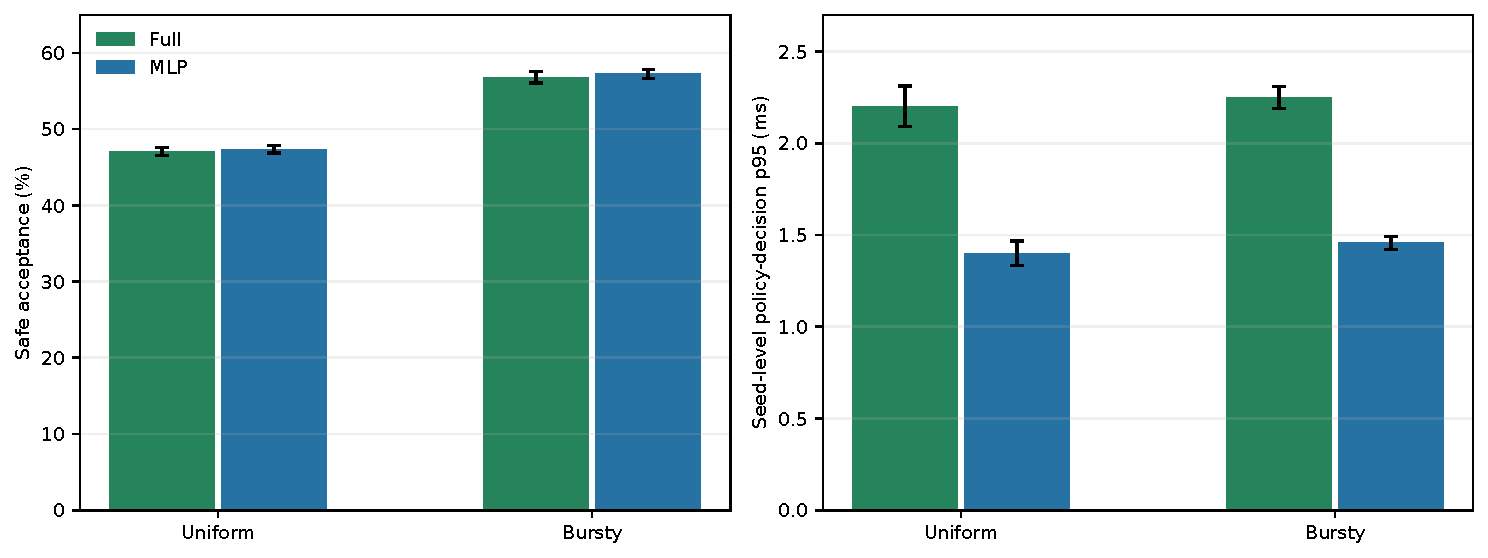
\includegraphics[width=0.94\textwidth]{figs/ablation_compute_cost.pdf}
\caption{\newrev{Acceptance and measured computation cost of Full and MLP ablation checkpoints on Vietnam. Bars show means and error bars show sample SD across 20 evaluation seeds. The right panel aggregates the per-seed p95 interval including normalization, inference, and simulator stepping; it excludes external controller actuation.}}
\label{fig:ablation_cost}
\end{figure*}

\newrev{Table~\ref{tab:timed_full_coverage} summarizes full-policy acceptance and timing across ten topology--workload conditions. Each condition includes 20 seeds and records zero admitted modeled hard violations. Workload and execution conditions also affect timing, so the differences cannot be attributed to substrate size alone.}
\begin{table}[t]
\centering
\caption{\newrev{Full-policy safe acceptance and decision timing (20 seeds; mean $\pm$ sample SD). Timing summarizes seed-level p95 values; it is not a pooled request-level p95.}}
\label{tab:timed_full_coverage}
{\color{ForestGreen}\scriptsize
\setlength{\tabcolsep}{3pt}
\resizebox{\columnwidth}{!}{%
\begin{tabular}{llrr}
\toprule
Network & Workload & Safe (\%) & p95 (ms) \\
\midrule
GEANT2 & Bursty & 80.52 $\pm$ 0.46 & 2.969 $\pm$ 0.032 \\
GEANT2 & Uniform & 71.32 $\pm$ 0.36 & 2.802 $\pm$ 0.079 \\
NSFNET & Bursty & 66.83 $\pm$ 0.56 & 2.242 $\pm$ 0.051 \\
NSFNET & Chaos & 52.34 $\pm$ 0.73 & 2.223 $\pm$ 0.063 \\
NSFNET & Heavy-tail & 51.43 $\pm$ 0.54 & 2.187 $\pm$ 0.055 \\
NSFNET & Uniform & 56.81 $\pm$ 0.69 & 2.173 $\pm$ 0.025 \\
Vietnam & Bursty & 56.83 $\pm$ 0.78 & 2.250 $\pm$ 0.062 \\
Vietnam & Chaos & 43.31 $\pm$ 0.84 & 1.986 $\pm$ 0.031 \\
Vietnam & Heavy-tail & 42.79 $\pm$ 0.70 & 2.105 $\pm$ 0.145 \\
Vietnam & Uniform & 47.10 $\pm$ 0.54 & 2.201 $\pm$ 0.111 \\
\bottomrule
\end{tabular}%
}}
\end{table}

\subsection{\newrev{Matched-Trace Candidate Pruning and Admission}}
\label{subsec:mask_admission}
\newrev{We evaluated seven ablation variants on Vietnam, NSFNET, and GEANT2 using four workloads (Uniform, Bursty, Heavy-tail, and a separately configured Chaos profile), 20 evaluation seeds, and 3,000 simulator steps per seed--workload cell. Run metadata records the checkpoint and observation normalizer for each variant. For each topology, workload, and seed, all variants use the same offered-request trace. Table~\ref{tab:mask_admission} reports the mean and sample standard deviation across the 80 seed--workload cells per topology; these values describe evaluation variation rather than uncertainty across independently trained policies.}

{\color{ForestGreen}
\begin{table*}[t]
\centering
\caption{Candidate pruning and local admission outcomes under matched traces (20 evaluation seeds across four workloads; mean $\pm$ sample SD over 80 seed--workload cells per topology, percentages).}
\label{tab:mask_admission}
\scriptsize
\begin{tabular}{llrrrr}
\toprule
Topology & Variant & Mask-pruned candidates & Runtime rejected & Admitted hard violations & Safe acceptance \\
\midrule
Vietnam & Full mask + admission & 84.20 $\pm$ 2.76 & 52.49 $\pm$ 5.71 & 0.00 $\pm$ 0.00 & 47.51 $\pm$ 5.71 \\
Vietnam & MLP + mask + admission & 83.61 $\pm$ 2.99 & 52.16 $\pm$ 5.75 & 0.00 $\pm$ 0.00 & 47.84 $\pm$ 5.75 \\
Vietnam & NoAdapt + mask + admission & 84.19 $\pm$ 2.72 & 52.56 $\pm$ 5.56 & 0.00 $\pm$ 0.00 & 47.44 $\pm$ 5.56 \\
Vietnam & No mask + admission & 0.00 $\pm$ 0.00 & 86.74 $\pm$ 2.25 & 0.00 $\pm$ 0.00 & 13.26 $\pm$ 2.25 \\
Vietnam & No mask + MSD admission off & 0.00 $\pm$ 0.00 & 86.75 $\pm$ 2.24 & 0.00 $\pm$ 0.01 & 13.25 $\pm$ 2.24 \\
Vietnam & Soft MSD, admission off & 0.00 $\pm$ 0.00 & 75.88 $\pm$ 1.30 & 0.07 $\pm$ 0.08 & 24.05 $\pm$ 1.28 \\
Vietnam & Soft MSD + admission & 0.00 $\pm$ 0.00 & 75.80 $\pm$ 1.36 & 0.00 $\pm$ 0.00 & 24.20 $\pm$ 1.36 \\
NSFNET & Full mask + admission & 80.94 $\pm$ 3.55 & 43.15 $\pm$ 6.18 & 0.00 $\pm$ 0.00 & 56.85 $\pm$ 6.18 \\
NSFNET & MLP + mask + admission & 80.56 $\pm$ 3.33 & 42.86 $\pm$ 6.01 & 0.00 $\pm$ 0.00 & 57.14 $\pm$ 6.01 \\
NSFNET & NoAdapt + mask + admission & 81.34 $\pm$ 3.36 & 43.38 $\pm$ 6.11 & 0.00 $\pm$ 0.00 & 56.62 $\pm$ 6.11 \\
NSFNET & No mask + admission & 0.00 $\pm$ 0.00 & 72.87 $\pm$ 3.43 & 0.00 $\pm$ 0.00 & 27.13 $\pm$ 3.43 \\
NSFNET & No mask + MSD admission off & 0.00 $\pm$ 0.00 & 72.87 $\pm$ 3.43 & 0.00 $\pm$ 0.00 & 27.13 $\pm$ 3.43 \\
NSFNET & Soft MSD, admission off & 0.00 $\pm$ 0.00 & 55.40 $\pm$ 6.35 & 0.00 $\pm$ 0.00 & 44.60 $\pm$ 6.35 \\
NSFNET & Soft MSD + admission & 0.00 $\pm$ 0.00 & 55.40 $\pm$ 6.35 & 0.00 $\pm$ 0.00 & 44.60 $\pm$ 6.35 \\
GEANT2 & Full mask + admission & 74.72 $\pm$ 4.72 & 29.29 $\pm$ 6.23 & 0.00 $\pm$ 0.00 & 70.71 $\pm$ 6.23 \\
GEANT2 & MLP + mask + admission & 73.95 $\pm$ 4.66 & 29.24 $\pm$ 6.26 & 0.00 $\pm$ 0.00 & 70.76 $\pm$ 6.26 \\
GEANT2 & NoAdapt + mask + admission & 75.26 $\pm$ 4.39 & 29.46 $\pm$ 6.25 & 0.00 $\pm$ 0.00 & 70.54 $\pm$ 6.25 \\
GEANT2 & No mask + admission & 0.00 $\pm$ 0.00 & 65.89 $\pm$ 3.29 & 0.00 $\pm$ 0.00 & 34.11 $\pm$ 3.29 \\
GEANT2 & No mask + MSD admission off & 0.00 $\pm$ 0.00 & 65.90 $\pm$ 3.29 & 0.00 $\pm$ 0.01 & 34.10 $\pm$ 3.29 \\
GEANT2 & Soft MSD, admission off & 0.00 $\pm$ 0.00 & 73.46 $\pm$ 2.35 & 0.01 $\pm$ 0.02 & 26.54 $\pm$ 2.36 \\
GEANT2 & Soft MSD + admission & 0.00 $\pm$ 0.00 & 73.40 $\pm$ 2.36 & 0.00 $\pm$ 0.00 & 26.60 $\pm$ 2.36 \\
\bottomrule
\end{tabular}
\end{table*}
}

{\color{ForestGreen}
\begin{table}[t]
\centering
\caption{\newrev{Proposed and admitted hard violations (\%; 720,000 simulator steps per variant across topologies, workloads, and seeds). CPU/RAM/BW/MSD proposal rates overlap; Union counts requests with any proposed hard violation, and Admitted reports admitted hard violations.}}
\label{tab:proposal_violations}
\scriptsize
\setlength{\tabcolsep}{3pt}
\resizebox{\columnwidth}{!}{%
\begin{tabular}{lrrrrrr}
\toprule
Variant & CPU & RAM & BW & MSD & Union & Admitted \\
\midrule
Full & 41.641 & 6.069 & 0.000 & 0.029 & 41.642 & 0.000 \\
MLP & 41.415 & 1.564 & 0.000 & 0.122 & 41.416 & 0.000 \\
NoMask + admission & 75.139 & 3.653 & 0.000 & 0.002 & 75.168 & 0.000 \\
NoMask + MSD admission off & 75.146 & 3.633 & 0.000 & 0.001 & 75.175 & 0.001 \\
SoftMSD + admission off & 68.214 & 2.863 & 0.000 & 0.328 & 68.271 & 0.025 \\
SoftMSD + admission on & 68.136 & 2.819 & 0.000 & 0.352 & 68.198 & 0.000 \\
NoAdapt & 41.798 & 5.685 & 0.000 & 0.000 & 41.799 & 0.000 \\
\bottomrule
\end{tabular}%
}
\end{table}
}

\newrev{Figure~\ref{fig:ablation_pruning} compares candidate pruning and safe acceptance. Candidate pruning is the per-step fraction of the flat $N^2$ action set removed before policy sampling. Runtime rejection and safe acceptance use offered, non-skipped requests as the denominator; admitted hard violations are the union of the modeled CPU, RAM, bandwidth, and MSD violations among admitted requests. The full policy prunes 74.72--84.20\% of candidates across the three topologies. The pooled ablation comprises 720,000 simulator steps per variant. On this evaluation, the no-mask variant proposed a hard-invalid action on 75.17\% of offered requests, compared with 41.64\% for the full policy; the admission check rejected these proposals, and no hard-invalid requests were admitted in either protected condition. Because the policies differ as well as the masks, this comparison does not isolate the causal effect of masking. Per-constraint proposal rates in Table~\ref{tab:proposal_violations} overlap; their union avoids double-counting requests. The MSD reward coefficient is $-50$. With the same NoMask checkpoint, disabling MSD admission admitted 9 MSD-invalid actions over the 720,000-step evaluation (0.00125\%); the SoftMSD checkpoint admitted 182 such actions (0.02528\%) with MSD admission disabled and none with it enabled. CPU, RAM, and bandwidth checks remained active in both MSD-admission-bypass conditions. Although paired variants receive the same offered trace, different admission decisions can change later states, so request outcomes are not per-request counterfactual pairs. The reported latency field measures simulated service latency, not policy-computation overhead. These results characterize the implemented simulator predicates and do not establish full-chain deployment or data-plane forwarding safety.}

\begin{figure*}[t]
\centering
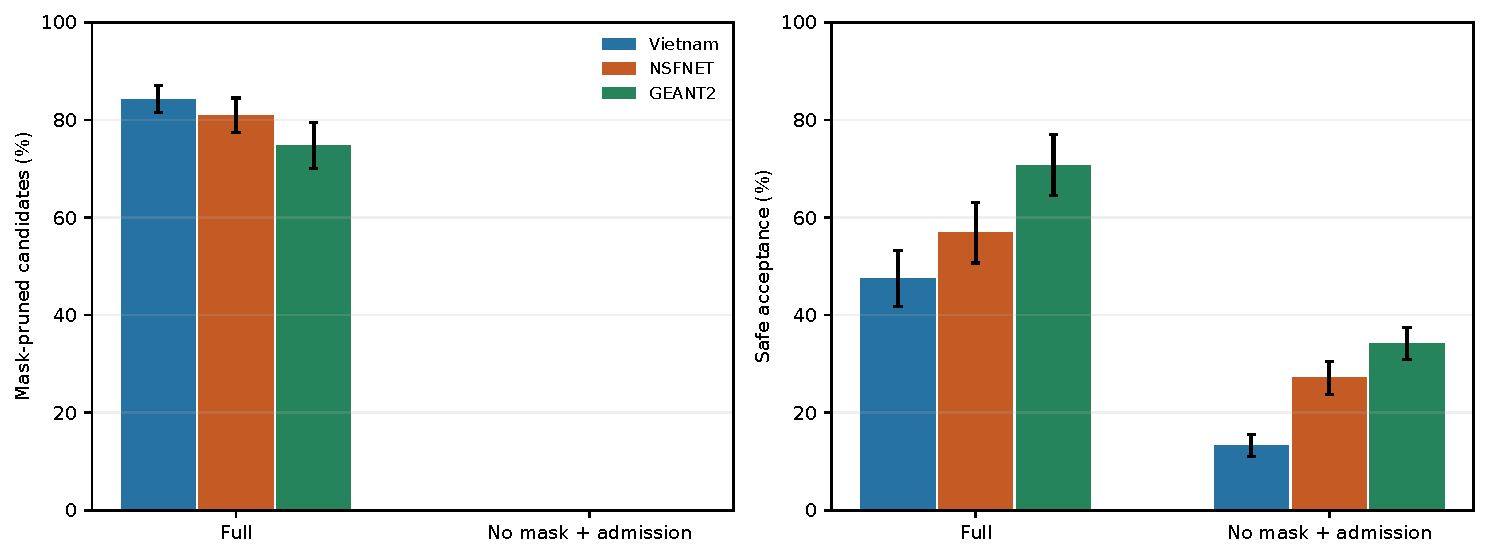
\includegraphics[width=0.94\textwidth]{figs/ablation_mask_admission.pdf}
\caption{\newrev{Candidate pruning and safe acceptance for Full and NoMask ablation variants with runtime admission enabled. Bars summarize 80 seed--workload cells per topology; error bars are sample SD across those cells. All six protected configurations recorded zero admitted hard violations. Distinct checkpoints and resulting state trajectories limit causal attribution to masking alone.}}
\label{fig:ablation_pruning}
\end{figure*}

\subsection{\newrev{Hardware-in-the-Loop Testbed Validation}}
\label{subsec:testbed_validation}
\newrev{Figure~\ref{fig:testbed_architecture_eval} shows the testbed architecture integrating the orchestration backend, policy engine, admission service, MicroK8s/Tekton lifecycle control, Mininet, BMv2 P4 switches, and SRv6 steering. The diagram describes the experimental infrastructure; quantitative validation requires the correlated execution evidence discussed below.}

\begin{figure*}[t]
    \centering
    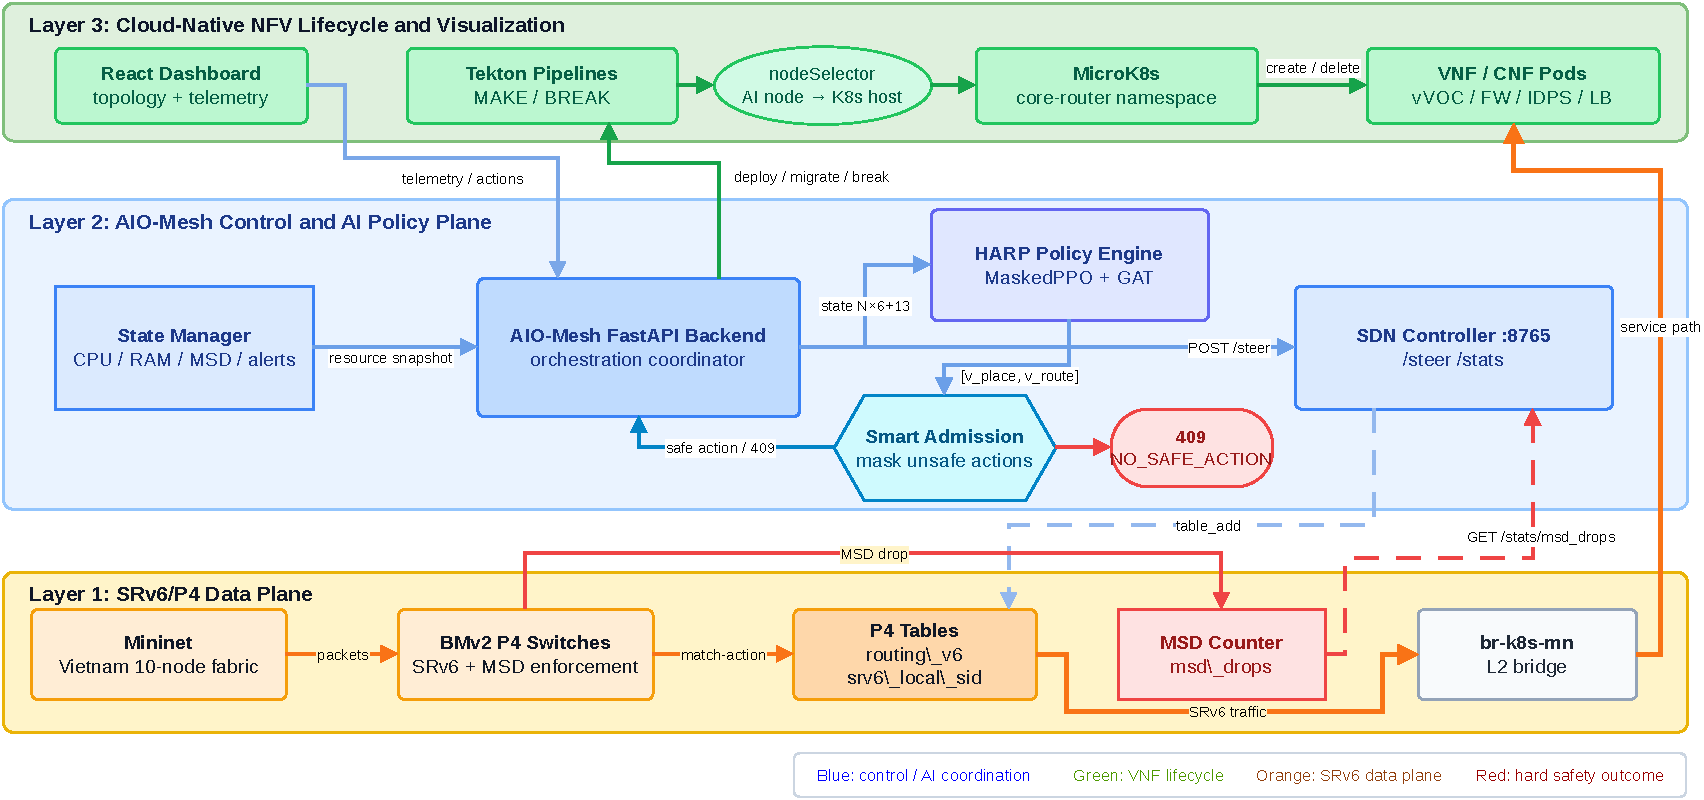
\includegraphics[width=\linewidth]{figs/testbed.pdf}
    \caption{\newrev{AIO-Mesh testbed architecture with MicroK8s, Tekton, Mininet, BMv2 P4 switches, SRv6 steering, and runtime admission control. The software-forwarding target and control interfaces define the scope of testbed validation.}}
    \label{fig:testbed_architecture_eval}
\end{figure*}

\newrev{Testbed validation distinguishes local admission, successful deployment, and observed forwarding. Deployment is established by lifecycle and controller confirmations; forwarding requires request-correlated packet or counter observations. The simulator acceptance and violation rates above measure local admission only. Extended stability and over-depth forwarding measurements are outside the quantitative results presented here.}

\newrev{Make-before-break ordering does not by itself establish zero packet loss or service continuity. Any result from BMv2 would characterize that software-forwarding target and should not be generalized to production ASIC performance.}

\subsection{\newrev{Scalability and Online Processing Overhead}}
\label{subsec:hardware_safe_admission}
\label{subsec:scalability_path_sensitivity}
\newrev{The load-sweep protocol evaluates the four protected algorithms at seven offered-intensity multipliers from 0.2 to 1.5 on Vietnam, NSFNET, and GEANT2, using 20 seeds and 3,000 simulator steps per seed and multiplier. At multipliers up to 1.0, the multiplier sets the request-arrival rate. Above 1.0, arrival rate is capped at 1.0 while CPU/RAM demand, requested SID depth, and TTL are scaled. We therefore interpret this protocol as a combined offered-intensity stress test rather than a pure arrival-rate sweep.}

\newrev{The load sweep comprises 3,360 seed-level policy trials across three substrates, seven intensities, and eight protected/unprotected modes. Figure~\ref{fig:load_sweep} shows all four protected policies; Table~\ref{tab:load_sweep_results} gives their safe acceptance at every intensity. Shaded bands are percentile-bootstrap 95\% intervals from 10,000 seed resamples. All protected trials recorded zero admitted modeled hard violations. Runtime rejection is the sum of the mutually exclusive CPU, RAM, MSD, bandwidth, and other rejection categories; the evaluation records include both admission modes and the per-constraint outcomes.}

\begin{figure*}[t]
\centering
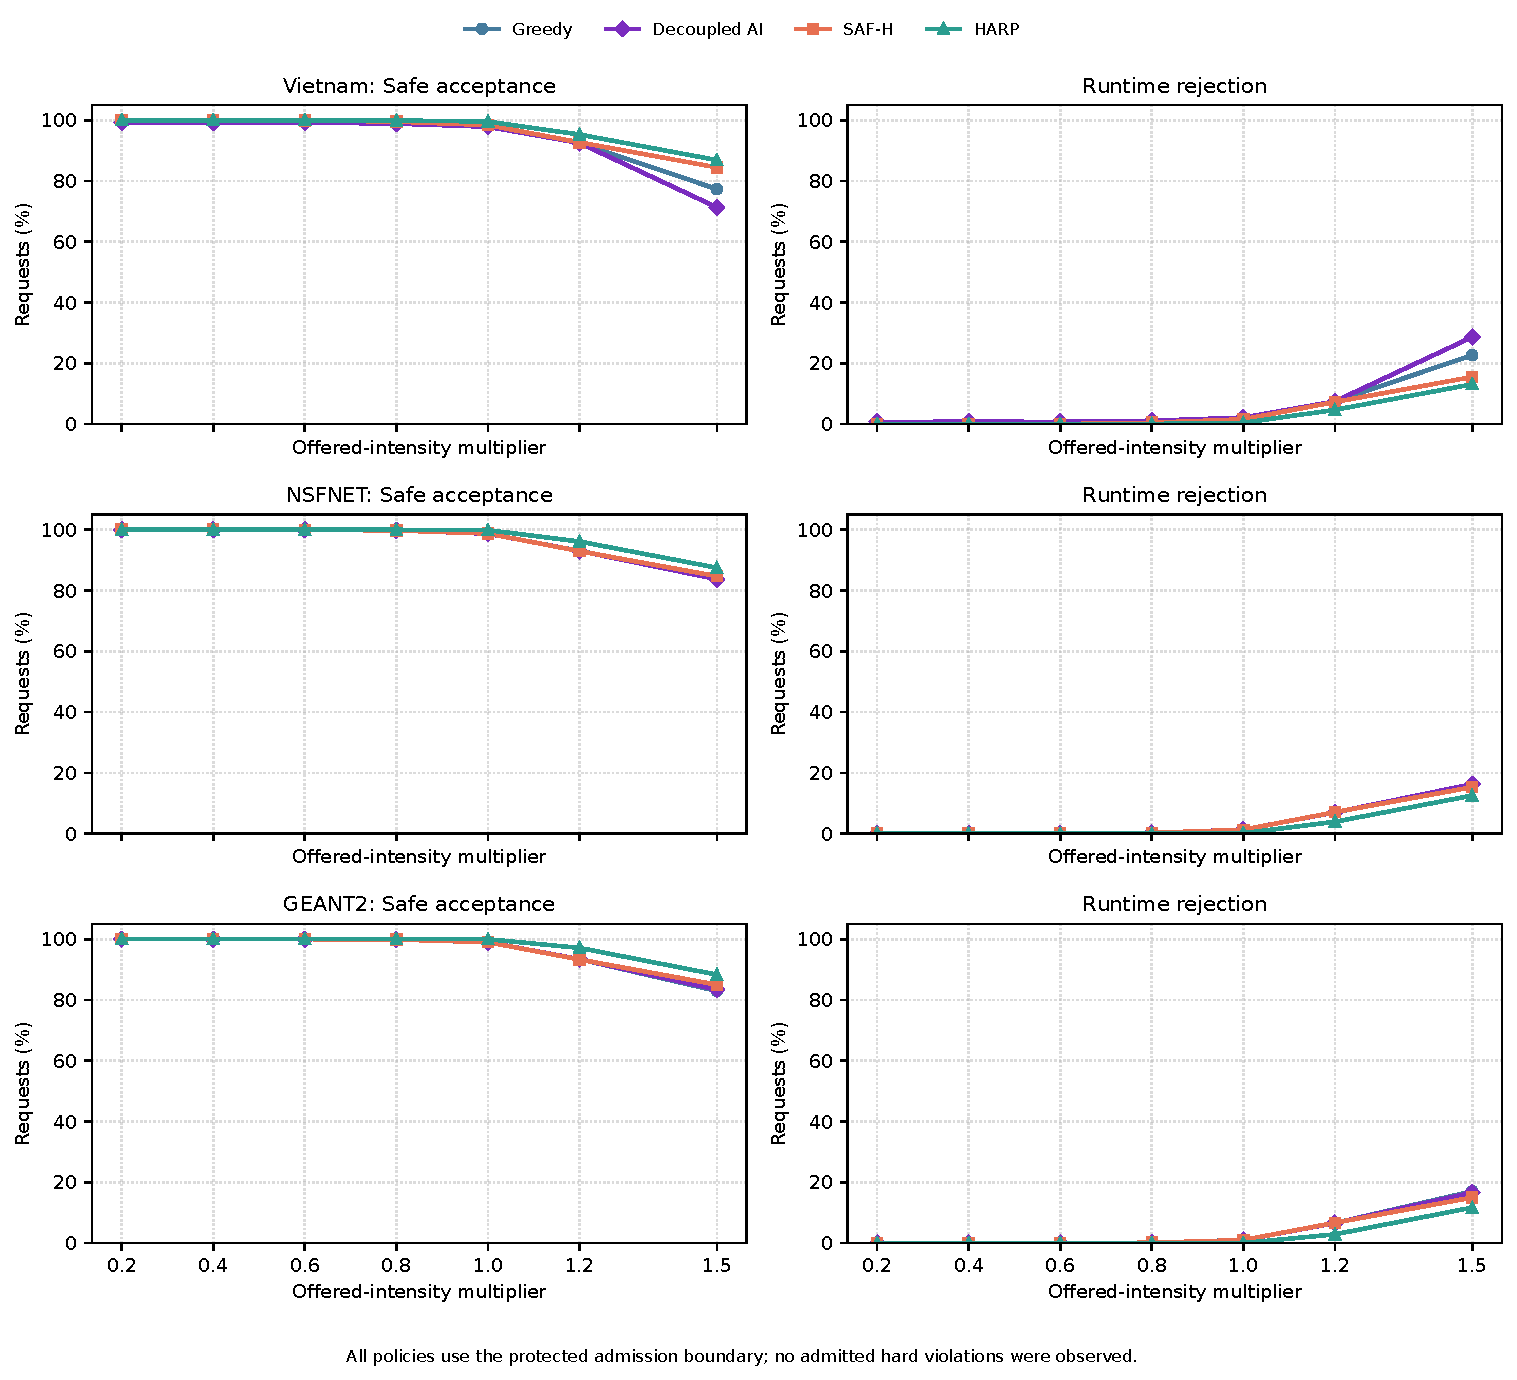
\includegraphics[width=0.97\textwidth]{figs/load_sweep_three_topologies.pdf}
\caption{\newrev{Current-code load sweep across Vietnam, NSFNET, and GEANT2. Left: safe acceptance; right: runtime rejection for the four protected policies. Lines show means over 20 seeds and shading shows bootstrap 95\% intervals. The offered-intensity multiplier changes arrival probability up to 1.0 and scales demand and TTL above 1.0; this is not a pure arrival-rate sweep. All protected admitted hard-violation rates were zero.}}
\label{fig:load_sweep}
\end{figure*}

\begin{table}[t]
\centering
\caption{\newrev{Protected-policy safe acceptance across the load sweep (\%; mean $\pm$ sample SD, 20 seeds). Load denotes offered intensity; DAI denotes Decoupled AI.}}
\label{tab:load_sweep_results}
\scriptsize
{\color{ForestGreen}
\setlength{\tabcolsep}{3pt}
\resizebox{\columnwidth}{!}{%
\begin{tabular}{llrrrr}
\toprule
Network & Load & Greedy & DAI & SAF-H & HARP \\
\midrule
Vietnam & 0.2 & 99.62 $\pm$ 0.20 & 99.26 $\pm$ 0.32 & 100.00 $\pm$ 0.00 & 100.00 $\pm$ 0.00 \\
Vietnam & 0.4 & 99.65 $\pm$ 0.17 & 99.20 $\pm$ 0.24 & 100.00 $\pm$ 0.02 & 100.00 $\pm$ 0.00 \\
Vietnam & 0.6 & 99.60 $\pm$ 0.22 & 99.24 $\pm$ 0.23 & 99.98 $\pm$ 0.04 & 100.00 $\pm$ 0.00 \\
Vietnam & 0.8 & 99.24 $\pm$ 0.20 & 98.87 $\pm$ 0.14 & 99.53 $\pm$ 0.12 & 99.93 $\pm$ 0.05 \\
Vietnam & 1.0 & 98.14 $\pm$ 0.19 & 97.85 $\pm$ 0.25 & 98.40 $\pm$ 0.18 & 99.56 $\pm$ 0.10 \\
Vietnam & 1.2 & 92.52 $\pm$ 0.25 & 92.52 $\pm$ 0.29 & 92.72 $\pm$ 0.19 & 95.29 $\pm$ 0.20 \\
Vietnam & 1.5 & 77.33 $\pm$ 0.26 & 71.35 $\pm$ 0.46 & 84.47 $\pm$ 0.23 & 86.88 $\pm$ 0.31 \\
NSFNET & 0.2 & 100.00 $\pm$ 0.00 & 100.00 $\pm$ 0.00 & 100.00 $\pm$ 0.00 & 100.00 $\pm$ 0.00 \\
NSFNET & 0.4 & 100.00 $\pm$ 0.00 & 100.00 $\pm$ 0.00 & 100.00 $\pm$ 0.00 & 100.00 $\pm$ 0.00 \\
NSFNET & 0.6 & 99.99 $\pm$ 0.03 & 99.99 $\pm$ 0.03 & 99.99 $\pm$ 0.03 & 100.00 $\pm$ 0.00 \\
NSFNET & 0.8 & 99.76 $\pm$ 0.11 & 99.76 $\pm$ 0.10 & 99.74 $\pm$ 0.13 & 99.99 $\pm$ 0.02 \\
NSFNET & 1.0 & 98.70 $\pm$ 0.17 & 98.69 $\pm$ 0.17 & 98.73 $\pm$ 0.16 & 99.86 $\pm$ 0.06 \\
NSFNET & 1.2 & 93.03 $\pm$ 0.16 & 93.00 $\pm$ 0.16 & 92.95 $\pm$ 0.29 & 96.11 $\pm$ 0.17 \\
NSFNET & 1.5 & 84.40 $\pm$ 0.25 & 83.73 $\pm$ 0.33 & 84.71 $\pm$ 0.16 & 87.47 $\pm$ 0.23 \\
GEANT2 & 0.2 & 100.00 $\pm$ 0.00 & 100.00 $\pm$ 0.00 & 100.00 $\pm$ 0.00 & 100.00 $\pm$ 0.00 \\
GEANT2 & 0.4 & 100.00 $\pm$ 0.00 & 100.00 $\pm$ 0.00 & 100.00 $\pm$ 0.00 & 100.00 $\pm$ 0.00 \\
GEANT2 & 0.6 & 99.99 $\pm$ 0.02 & 99.99 $\pm$ 0.02 & 99.99 $\pm$ 0.02 & 100.00 $\pm$ 0.00 \\
GEANT2 & 0.8 & 99.89 $\pm$ 0.07 & 99.89 $\pm$ 0.07 & 99.88 $\pm$ 0.08 & 100.00 $\pm$ 0.00 \\
GEANT2 & 1.0 & 98.99 $\pm$ 0.13 & 99.01 $\pm$ 0.12 & 99.00 $\pm$ 0.13 & 99.99 $\pm$ 0.02 \\
GEANT2 & 1.2 & 93.42 $\pm$ 0.24 & 93.42 $\pm$ 0.24 & 93.32 $\pm$ 0.24 & 97.12 $\pm$ 0.18 \\
GEANT2 & 1.5 & 82.96 $\pm$ 0.26 & 83.39 $\pm$ 0.31 & 85.01 $\pm$ 0.22 & 88.32 $\pm$ 0.25 \\
\bottomrule
\end{tabular}%
}}
\end{table}

\newrev{HARP's advantage over SAF-H emerges as occupancy and demand increase in this protocol. At intensity 1.2, safe acceptance is 95.29\% versus 92.72\% on Vietnam, 96.11\% versus 92.95\% on NSFNET, and 97.12\% versus 93.32\% on GEANT2. At intensity 1.5, the corresponding HARP--SAF-H differences are 2.408, 2.757, and 3.312 percentage points. For GEANT2 at 1.2, the paired difference is 3.803 points (bootstrap 95\% CI [3.688, 3.918]). All nine comparisons at intensities 1.0, 1.2, and 1.5 favor HARP with Holm-adjusted $p=4.01\times10^{-5}$ across the 21 topology--intensity tests. These estimates concern evaluation-seed variation conditional on fixed checkpoints and the offered workload, not independently trained policy populations.}

\newrev{Acceptance is substantially higher under the shorter, topology-scaled TTL protocol than in the three-workload stress benchmark. The favorable sweep results therefore identify a workload regime in which HARP improves safe acceptance relative to SAF-H; they do not establish an advantage under long-lived stress traffic or explain individual rejections as globally infeasible.}

\newrev{A separate active-chain experiment initializes 0, 25, 50, or 100 long-lived background chains before each 3,000-step Bursty evaluation. Each chain reserves 2 CPU units, 2 RAM units, and 20 bandwidth units, with round-robin placement. The run covers 20 seeds and all four protected algorithms on Vietnam, NSFNET, and GEANT2. Table~\ref{tab:active_chain_stress} compares protected HARP and SAF-H; the reported values are mean safe acceptance with sample standard deviation across seeds. Admitted modeled hard violations were zero for all protected algorithms in every tested condition. HARP's safe acceptance declined as background occupancy increased, while remaining above SAF-H in these simulator conditions.}

{\color{ForestGreen}
\begin{table}[t]
\centering
\caption{Safe acceptance under long-lived background-chain occupancy (20 seeds; mean $\pm$ sample SD, percentages).}
\label{tab:active_chain_stress}
\scriptsize
\setlength{\tabcolsep}{3pt}
\resizebox{\columnwidth}{!}{%
\begin{tabular}{lrrr}
\toprule
Network & Chains & HARP & SAF-H \\
\midrule
Vietnam & 0 & 99.56 $\pm$ 0.10 & 98.40 $\pm$ 0.18 \\
Vietnam & 25 & 99.19 $\pm$ 0.12 & 97.62 $\pm$ 0.18 \\
Vietnam & 50 & 98.61 $\pm$ 0.12 & 96.69 $\pm$ 0.23 \\
Vietnam & 100 & 97.05 $\pm$ 0.20 & 94.38 $\pm$ 0.17 \\
NSFNET & 0 & 99.86 $\pm$ 0.06 & 98.73 $\pm$ 0.16 \\
NSFNET & 25 & 99.66 $\pm$ 0.13 & 98.19 $\pm$ 0.15 \\
NSFNET & 50 & 99.42 $\pm$ 0.12 & 97.56 $\pm$ 0.14 \\
NSFNET & 100 & 98.63 $\pm$ 0.16 & 95.96 $\pm$ 0.19 \\
GEANT2 & 0 & 99.99 $\pm$ 0.02 & 99.00 $\pm$ 0.13 \\
GEANT2 & 25 & 99.97 $\pm$ 0.03 & 98.75 $\pm$ 0.16 \\
GEANT2 & 50 & 99.93 $\pm$ 0.05 & 98.47 $\pm$ 0.12 \\
GEANT2 & 100 & 99.80 $\pm$ 0.08 & 97.69 $\pm$ 0.18 \\
\bottomrule
\end{tabular}%
}
\end{table}
}

\newrev{Decision latency and actuation latency are distinct quantities. The active-chain experiment varies pre-existing simulated occupancy, but it does not isolate live request concurrency or measure a complete per-request interval from state construction to controller handoff. Accordingly, we make no quantitative end-to-end latency or scalability claim. Component averages cannot be interpreted as end-to-end tail latency or completed throughput.}

\subsection{\newrev{Operational Interpretation, Overhead, and Limitations}}
\label{subsec:operational_interpretation}
\newrev{The policy comparison depends on the resource-pressure regime. SAF-H achieves higher acceptance in all six Vietnam and NSFNET stress conditions, and in GEANT2 Chaos; HARP improves GEANT2 Burst-surge acceptance by 0.963 percentage points, while the Elephant-stress difference is inconclusive. Under the shorter-lifetime load-sweep protocol, HARP instead exceeds SAF-H on all three substrates at intensities 1.0--1.5, reaching gains of 2.408--3.312 points at 1.5. The background-occupancy experiment also favors HARP within its protocol. Together, these findings support workload-specific policy selection within a common admission interface.}

\newrev{Acceptance gains must also be weighed against computation. In the Vietnam ablation, the MLP variant achieves slightly higher mean safe acceptance and lower mean seed-level decision p95 than the full GAT policy under both Uniform and Bursty traffic (Figure~\ref{fig:ablation_cost}). This comparison provides no evidence that graph encoding improves the measured acceptance--cost tradeoff in those conditions. A direct HARP--SAF-H cost comparison under the same execution conditions is needed to determine whether the load-sweep acceptance gains justify learned inference. The common admission boundary permits either policy to be selected without assigning the enforcement outcome to that policy.}

\newrev{Several limitations bound these findings. The evaluated substrates use complete latency-derived graphs, and fixed-checkpoint seed variation does not measure training uncertainty or convergence. An exhaustive feasibility oracle is absent, so rejection rates combine genuine resource pressure with any missed feasible alternatives. Simulator timing excludes external actuation and live controller concurrency. Finally, pair-level resource and MSD checks do not certify a complete service-chain realization: telemetry validity, installed SID-path correspondence, cross-controller consistency, and packet-level migration continuity require separate operational evidence.}

\section{Conclusion}
\label{sec:conclusion}
\newrev{AIO-Mesh organizes candidate selection, local admission, lifecycle control, and programmable steering around a replaceable policy interface. Across the evaluated simulator conditions, all protected policies admit zero modeled hard violations. The ablation distinguishes this enforcement outcome from candidate quality: the full mask prunes 74.72--84.20\% of candidate actions, while disabling MSD admission permits violations that a soft reward penalty alone does not eliminate.}

\newrev{HARP's acceptance advantage is workload-dependent. SAF-H leads in seven of nine stress conditions, HARP leads in GEANT2 Burst surge, and one comparison is inconclusive after Holm correction. In the separate load sweep, HARP gains 2.408--3.312 percentage points at intensity 1.5 across the three substrates. These results motivate selecting policies by workload and computational cost while retaining independent admission. Extending the demonstrated pair-level checks to deployed service chains requires validation of realization, actuation, and forwarding.}


\section*{Declaration of Competing Interest}
The authors declare that they have no known competing financial interests or personal relationships that could have appeared to influence the work reported in this paper.

\section*{Funding} 
\noindent This work was supported by the Ministry of Science and Technology of Vietnam through the National Science and Technology Program, under Project No.~KC.01.06/21-30.

\section*{Data and Code Availability}
\newrev{The project source code is available at the repository below. The exact request traces, model checkpoints, run manifests, and per-seed records supporting the simulation results are available from the corresponding author upon reasonable request:}
\url{https://github.com/uet-dis/AIO-Mesh/}.

\section*{Declaration of Generative AI and AI-Assisted Technologies in the Writing Process}
During the preparation of this work, the authors used generative AI and AI-assisted technologies to refine the scientific prose, improve readability, and polish LaTeX formatting. After using these technologies, the authors thoroughly reviewed and edited the content as needed and take full responsibility for the content of the published article.

\section*{CRediT Authorship Contribution Statement}
\textbf{Hanh P. Du}: Conceptualization, Methodology, Formal analysis, Validation, Writing -- original draft.
\textbf{Hung D. Hoang}: Software, Investigation, Testbed implementation, Visualization, Validation, Writing -- original draft.
\textbf{Thu H. Le}: Software, Data curation, Experimental evaluation, Visualization, Writing -- review \& editing.
\textbf{Tuan X. Le}: Software, Validation, Writing -- review \& editing.
\textbf{Giang L. Nguyen}: Formal analysis, Validation, Writing -- review \& editing.
\textbf{Hoa N. Nguyen}: Conceptualization, Methodology, Supervision, Project administration, Funding acquisition, Writing -- review \& editing.

\bibliographystyle{elsarticle-num}
\bibliography{refs}

\end{document}
